\chapter{One-dimensional finite-volume methods}
\label{chp-1d-fv}

\theoremstyle{plain}
\newtheorem{lema}{Lemma}[chapter]

\theoremstyle{plain}
\newtheorem{prop}{Proposition}[chapter]

\theoremstyle{plain}
\newtheorem{thrm}{Theorem}[chapter]

\theoremstyle{plain}
\newtheorem{remark}{Remark}[chapter]

\theoremstyle{plain}
\newtheorem{corollary}{Corollary}[chapter]

\theoremstyle{plain}
\newtheorem{definition}{Definition}[chapter]


The aim of this Chapter is to provide a detailed description of one-dimensional (1D) 
finite-volume (FV) schemes within a Semi-Lagrangian (SL) framework, specifically applied to 
the 1D advection equation.
These schemes are also known as flux-form Semi-Lagrangian schemes, and they allow for time steps beyond the 
Courant-Friedrichs-Lewy (CFL) condition while preserving the total mass.
FV-SL schemes have been explored in the literature since the work of  \citet{leveque:1985},
which extended the finite-volume schemes from \citet{godunov:1959}  to accommodate larger time steps.
This approach has been further investigated in the literature (cf. e.g. \citet{lin:1996,leonard:1996}).
We are going to focus on the linear advection equation because in FV3 the horizontal dynamics
are solved using flux advection operators to compute the fluid density, absolute vorticity, 
and the kinetic energy \citep{lin:1997,putmanthesis:2007, harris:2013, harris:2021}.
The boundary conditions are assumed to be periodic for simplicity.

To introduce the FV-SL schemes, we begin by discretizing the spatial and temporal domains into uniform grids.
Subsequently, the FV-SL schemes involve three steps.
The first step involves computing the departure points of the spatial grid edges.
The second step, known as reconstruction, utilizes the grid cell average values to
determine a piecewise function within each cell. This piecewise function approximates the
values of the advected quantity and ensures the preservation of its local mass within each grid cell.
The third step involves updating the fluxes at the grid edges by integrating the reconstruction function 
over a domain that extends from the departure point of the grid edge to the grid edge itself.

The first step of FV-SL schemes can be accomplished by integrating an ordinary differential
equation (ODE) backward in time.
The second step is performed using the Piecewise-Parabolic Method (PPM) proposed by \citet{colella:1984}.
As the name suggests, PPM employs piecewise-parabolic functions.
The third and final step is computed easily, as the reconstruction functions consist of parabolas that preserve the local mass.

It is worth noting that the reconstruction function can be constructed using functions other than parabolas.
In fact, PPM can be seen as an
extension of the Piecewise-Linear method proposed by \citet{vanleer:1977}, which,
in turn, was inspired by the Piecewise-Constant method introduced by \citet{godunov:1959}. 
Additionally, other schemes inspired by PPM have been proposed in the literature utilizing
higher-order polynomials, such as quartic polynomials \citep{white:2008}. For a
comprehensive review of general piecewise-polynomial reconstruction, we recommend
referring to the technical report by \citet{engwirda:2016}, \citet{lauritzen:2011}, and the
references therein.

The PPM approach has become popular in the literature for gas dynamics simulations, astrophysical 
phenomena modeling \citep{woodward:1986}, and later on atmospheric simulations \citep{carpenter:1990}. 
Indeed, PPM has been implemented in the FV3 dynamical core on its latitude-longitude grid \citep{lin:2004}
and cubed-sphere \citep{putman:2007} versions.
Although many other shapes for the basis functions and higher-order schemes are available in the literature, 
\citet{harris:2021} points out that the PPM scheme suits the needs of FV3 well. It is a flexible method that
can be modified to ensure low diffusivity or shape preservation, for example.
Additionally, a finite-volume numerical method usually requires monotonicity constraints, which, according 
to Godunov's order barrier theorem \citep{wesseling:2001}, limits the order of convergence to at most 1. 
Therefore, a higher-order scheme needs to strike a well-balanced trade-off between increasing computational 
cost and potential benefits.

This Chapter begins with a basic review of one-dimensional advection equation in the integral form
in Section \ref{chp-adv1d-sec1}. In Section \ref{chp-adv1d-sec2-fvsl}, we establish the framework for general
one-dimensional finite-volume Semi-Lagrangian schemes. Section \ref{chp-adv1d-sec-dp} presents
methods for computing the departure point. The PPM reconstruction is described in Section \ref{chp-adv1d-sec-recon},
while Subsection \ref{chp-adv1d-sec-hord8} introduces a different approach to ensure the monotonicity of parabolas.
Section \ref{chp-adv1d-sec-flux} focuses on the description and investigation of the PPM flux computation.
Section \ref{chp-adv1d-sec-numerical-exp}
presents numerical results using the PPM scheme for the advection equation.
Finally, Section \ref{chp-adv1d-sec-conclusion} presents some concluding remarks.
The application of PPM to solve two-dimensional problems will be addressed in Chapter \ref{chp-2d-fv}.

\section{One-dimensional advection equation in the integral form}
\label{chp-adv1d-sec1}

\subsection{Notation}
\label{chp-adv1d-sec-not}
Before introducing the FV-SL schemes, let us establish some notation by introducing
the concepts of a $\Delta x$-grid, a $\Delta t$-temporal grid, and the
$(\Delta x, \Delta t, \lambda)$-discretization, as well as the concept of grid function/winds.
In this Chapter, we will use the notation $\Omega=[a,b]$ to represent the interval under consideration,
and $\nu$ to represent a non-negative integer indicating the number of ghost cell layers in each boundary.
We also use the notations $\mathbb{R}^{N}_{\nu}:=\mathbb{R}^{N+2\nu}$ and
$\mathbb{R}^{N+1}_{\nu}:=\mathbb{R}^{N+1+2\nu}$.
\begin{definition}[$\Delta x$-grid]\label{chp-adv1d-def-dxgrid}
	For a given interval $\Omega$ and a positive real number $\Delta x$ such that 
    $\Delta x = (b-a)/N$ for some positive integer $N$, 
	we say that $\Omega_{\Delta x}= \{X_i \}_{i=-\nu+1}^{N+\nu}$ is a $\Delta x$-grid for $\Omega$ if
	\begin{align*}
        X_i = [x_{i-\frac{1}{2}},x_{i+\frac{1}{2}}] = [a+(i-1)\Delta x, a+i\Delta x],
    \end{align*}
	and $\Delta x = x_{i+\frac{1}{2}} - x_{i-\frac{1}{2}}$. 
	Each $X_i$ is referred to as a control volume or cell, and $x_{i-\frac{1}{2}}$ and 
	$x_{i+\frac{1}{2}}$ are the edges of the control volume $X_i$.
	The cell centroid is defined by
    \begin{align*}
    x_i = \frac{1}{2}(x_{i+\frac{1}{2}} + x_{i-\frac{1}{2}}),\quad \forall i = -\nu+1, \ldots, N+\nu,
    \end{align*}
	and $\Delta x$ is the cell length.
\end{definition}
\begin{remark}
If $1 \leq i \leq N$, we refer to $i$ as an interior index;
otherwise, $i$ is considered a ghost cell index and we say the $X_i$ is a ghost cell.
\end{remark}

\begin{figure}[!htb]
	\centering
	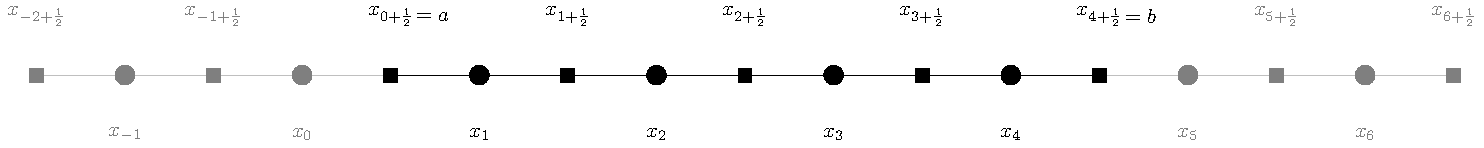
\includegraphics[width=1\linewidth]{1d_grid}
	\caption{Illustration of a $\Delta x$-grid with $N=4$ cells in its interior (in black) 
         and $\nu=2$ ghost cell layers (in gray).
	 The edges are denoted by squares and the cell centroids are denoted using circles.\label{chp-adv1d-sec1-grid1d}}
\end{figure}

\begin{definition}[$\Delta t$-temporal grid]
	For a given interval $[0,T]$ and a positive real number $\Delta t$ such that $\Delta t = T/N_T$
    for some positive integer $N_T$, we say that  $T_{\Delta T}= \{T_n\}_{n=0}^{N_T}$ a $\Delta t$-temporal grid for $[0,T]$ if
    \begin{align*}
	T_n = [t^n, t^{n+1}], \quad t^n = n\Delta t, \quad \Delta t = \frac{T}{N_T}, \quad \forall n = 0, \ldots, N_T.
    \end{align*}
    In this context, we also define $t^{n+\frac{1}{2}} = \frac{t^n+t^{n+1}}{2}$.
\end{definition}

\begin{definition}[$(\Delta x,\Delta t, \lambda)$-discretization]
\label{chp-adv1d-def-dxtimegrid}
	Given $\Omega \times [0,T]$ and positive real numbers $\Delta x$ and $\Delta t$,
    we say that $(\Omega_{\Delta x}, T_{\Delta t})$ is a $(\Delta x, \Delta t, \lambda)$-discretization 
    of $\Omega \times [0,T]$ if $\Omega_{\Delta x}$ is a $\Delta x$-grid for $\Omega$, 
    ${T}_{\Delta t}$ is a $\Delta t$-temporal grid for $[0,T]$, and $\frac{\Delta t}{\Delta x} = \lambda$.
\end{definition}
\begin{remark}
	Whenever we refer to a $\Delta x$-grid, a $\Delta t$-temporal grid, or a $(\Delta x, \Delta t, \lambda)$-discretization, 
	$X_i$, $N$, $t^n$, and $N_T$ are assumed to be implicitly defined.
\end{remark}
Next, we introduce the definitions of grid functions at cell centroids and edges.
\begin{definition}[$\Delta x$-grid function]
	For a $\Delta x$-grid, we say that $Q$ is a $\Delta x$-grid function if
	$Q = (Q_{-\nu+1}, \ldots, Q_{N+\nu}) \in \mathbb{R}^{N}_{\nu}$.
\end{definition}
\begin{definition}[$\Delta x$-grid wind]
	For a $\Delta x$-grid, we say that $u$ is a $\Delta x$-grid wind if
	$u = (u_{-\nu+\frac{1}{2}}, \ldots, u_{N+\nu+\frac{1}{2}}) \in \mathbb{R}^{N+1}_{\nu}$.
\end{definition}
The definition of a $\Delta x$-grid wind is based on the Arakawa grids \citep{arakawa:1977}.
Considering functions $q, u: \Omega \times[0,T] \to \mathbb{R}$ and a $(\Delta x,\Delta t, \lambda)$-discretization
of $\Omega \times[0,T]$, we introduce the grid functions $q^n \in \mathbb{R}^{N}_{\nu}$ and $u^n \in \mathbb{R}^{N+1}_{\nu}$. 
Here, ${q}^n_{i} = {q}(x_i, t^{n})$ and $u^n_{i+\frac{1}{2}} = u(x_{i+\frac{1}{2}},t^n)$.
These grid functions represent the discrete values of $q$ and $u$ at the cell centroids and edges, respectively,
for each time level $t^n$  (Figure \ref{chp-adv1d-sec1-grid1d-function}).


In this Chapter, our focus lies on periodic grid functions.
We define a $\Delta x$-grid function $Q$ as periodic if it satisfies the following conditions:
\begin{align*}
    Q_{i} &= Q_{N+i}, \quad i=-\nu+1, \ldots, 0,\\
    Q_{i} &= Q_{i-N}, \quad i=N+1, \ldots, N+\nu.
\end{align*}
Similarly, we define a $\Delta x$-grid wind as periodic if it meets the following requirements:
\begin{align*}
    u_{i-\frac{1}{2}} &= u_{N+i+\frac{1}{2}} , \quad i=-\nu, \ldots, -1,\\
    u_{i+\frac{1}{2}} &= u_{i+\frac{1}{2}-N} , \quad i=N+1, \ldots, N+\nu.
\end{align*}
We use the notation $\mathbb{P}^{N}_{\nu}$ and $\mathbb{P}^{N+1}_{\nu}$ to
represent the spaces of periodic $\Delta x$-grid functions and winds, respectively.
\begin{figure}[!htb] 
\centering 
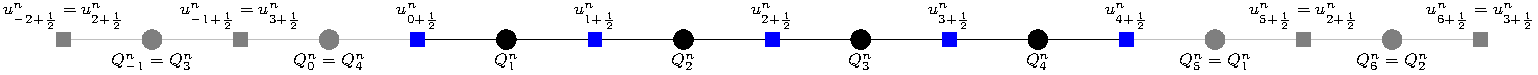
\includegraphics[width=1\linewidth]{1d_grid_function} 
\caption{Illustration of $\Delta x$-grid function $Q$ (black circles)
and a $\Delta x$-grid wind $u$ (blue squares) and its ghost cell
values (in gray) assuming periodicity.\label{chp-adv1d-sec1-grid1d-function}}
\end{figure}

Given $Q \in \mathbb{P}^{N}_{\nu}$, we define the $p$-norm as
\begin{equation}
	\label{chp-adv1d-sec-not1}
	\|Q\|_{p,\Delta x}=
	\begin{cases}
		\bigg( \sum_{i=1}^{N} |Q_i|^p \bigg)^{\frac{1}{p}} & \text{if } 1\leq p < \infty,\\
		\max_{i=1, \ldots, N}{|Q_i|} & \text{if } p=\infty,
	\end{cases}
\end{equation}
which is indeed a norm for periodic grid functions.
Using a similar notation as in \citet{engwirda:2016}, we define the stencil and a grid function evaluated on a stencil as follows.
\begin{definition}[Stencil]
	For a $\Delta x$-grid, and each $i = 0, \ldots, N$, we define a stencil as a set of the form
	$\mathcal{S}_{i+\frac{1}{2}} = \{i-r+1, \ldots, i-1, i, i+1, \ldots, i+s\} \subset\{-\nu+1, \ldots, N+\nu\}$.
\end{definition}
\begin{definition}[Grid function restricted to a stencil]
	For a $\Delta x$-grid, a stencil $\mathcal{S}_{i+\frac{1}{2}}$,
	 and a $\Delta x$-grid function $Q$, we define $Q(\mathcal{S}_{i+\frac{1}{2}}) = (Q_k)_{k \in \mathcal{S}_{i+\frac{1}{2}}}$.
\end{definition}
These definitions provide the necessary notation for describing grid functions and their evaluations on stencils.
To achieve a more compact notation in some situations, we introduce the centered difference notation:
\begin{equation}
    \label{chp-adv1d-sec-adv-eq5}
	\delta_x {g}(x_i,t) = 
	{g}(x_{i+\frac{1}{2}},t) - 
	{g}(x_{i-\frac{1}{2}},t),
\end{equation}
for any function $g: \Omega \times [0,T] \to \mathbb{R}$.
Additionally, we introduce the average value of $q$ in the $i$-th control volume at time $t$, denoted as ${Q}_i(t)$, defined by:
\begin{equation}
	\label{chp-adv1d-sec1-not2}
	{Q}_i(t) = \frac{1}{\Delta x} \int_{x_{i-\frac{1}{2}}}^{x_{i+\frac{1}{2}}} {q}(x,t) \,dx.
\end{equation}
Moreover, we define the $\Delta x$-grid function of average values as $Q(t) = (Q_i(t))_{i=-\nu+1}^{N+\nu}$.
Here, $Q_i(t)$ represents the average value of $q$ in the $i$-th control volume at time $t$.

For the consideration of periodic boundary conditions, we can define spaces of periodic functions over 
the interval $\Omega$ as follows:
\begin{align*}
	\mathcal{S}_P(\Omega) &= \{q:\mathbb{R}\times[0,+\infty[\to \mathbb{R}: q(x+b-a,t)=q(x,t), \quad \forall x \in \mathbb{R}, \quad t\geq0\}.
\end{align*}
Similarly, the space of $k$-times periodically differentiable functions $\mathcal{C}_P^k(\Omega)$ can be defined as:
\begin{align*}
	\mathcal{C}_P^k(\Omega) &= \mathcal{S}_P(\Omega)\cap \mathcal{C}^k(\mathbb{R}\times[0,\infty[),
\end{align*}
where $\mathcal{C}^k(\mathbb{R}\times[0,+\infty[)$ denotes the space of functions that are $k$ 
times continuously differentiable in both the spatial and temporal variables.
In summary, $\mathcal{S}_P(\Omega)$ represents the space of periodic functions, and $\mathcal{C}_P^k(\Omega)$
represents the space of $k$-times periodically differentiable functions over the interval $\Omega$ subject to periodic boundary conditions.

\subsection{The 1D advection equation}
In this Section, we will derive the integral form of the 1D advection equation with periodic boundary conditions over the interval $\Omega$.
What is going to be presented here follows \citet{leveque:1990,leveque:2002} closely.
The conservative advection equation with periodic boundary conditions is given by the following PDE:
\begin{equation}
	\label{chp-adv1d-sec-adv-eq1}
	\begin{cases}
		[{\partial_t q} + {\partial_x (uq)}](x, t)
		= 0, \quad \forall (x,t) \in \mathbb{R}\times ]0, +\infty[,\\
		{q}(a, t) = {q}(b, t), \quad \forall t\geq 0,\\
		q_0(x) = q(x,0), \quad \forall x \in \Omega.
	\end{cases}
\end{equation}
Here, $q \in \mathcal{C}_P^1{(\Omega)}$ represents the advected quantity density \citep{zerroukat:2006}, and $u \in \mathcal{C}_P^1{(\Omega)}$ represents the velocity or wind.
We will focus on Equation \eqref{chp-adv1d-sec-adv-eq1} over the domain $D = \Omega\times[0,T]$, where $T>0$ is a finite time.
A strong or classical solution to the advection equation is defined as a function ${q}\in\mathcal{C}^1_P(\Omega)$ 
and satisfies Equation \eqref{chp-adv1d-sec-adv-eq1}.
In order to deduce the integral form of Equation \eqref{chp-adv1d-sec-adv-eq1}, we consider
$[x_1, x_2]\times[t_1,t_2]\subset D$. 
Integrating Equation \eqref{chp-adv1d-sec-adv-eq2} over $[x_1, x_2]$, we obtain:
\begin{equation}
    \label{chp-adv1d-sec-adv-eq2}
	\frac{d}{dt} \int_{x_1}^{x_2} q(x,t) \,dx =  
	-({(uq)}(x_2,t) - {(uq)}(x_1,t)) ,
\end{equation}
and integrating Equation \eqref{chp-adv1d-sec-adv-eq2} over $[t_1,t_2]$, we get
\begin{equation}
    \label{chp-adv1d-sec-adv-eq3}
    \int_{x_1}^{x_2} q(x,t_2) \,dx=  \int_{x_1}^{x_2} q(x,t_1)
	-\bigg( \int_{t_1}^{t_2} 
	{(uq)}(x_2, t) \,dt - 
	\int_{t_1}^{t_2}{(uq)}(x_1, t) \,dt \bigg).
\end{equation}
The presented problem, Problem \ref{chp-adv1d-sec2-prob1}, aims to find a solution, called weak solution, to the advection equation
in its integral form, considering the given initial condition (IC) ${q}_0$ and velocity function $u$.

\theoremstyle{plain}
\newtheorem{prob}{Problem}[chapter]
\begin{prob}
	\label{chp-adv1d-sec2-prob1}
	Given an IC ${q}_0$ and a velocity function $u$  we would like to find a weak solution ${q}$
	of the advection equation in the integral form:
	\begin{equation*}
	        \int_{x_1}^{x_2} {q}(x, t_2) \,dx =
       		\int_{x_1}^{x_2} {q}(x, t_1) \,dx +
        	\int_{t_1}^{t_2} {(uq)}(x_1, t) \,dt -
		\int_{t_1}^{t_2}{(uq)}(x_2, t) \,dt ,
	\end{equation*}
	$\forall [x_1, x_2]\times[t_1, t_2] \subset \Omega \times [0,T]$,
	and
	${q}(x,0) = {q}_0(x)$, $\forall x \in \Omega$, $q(a,t)=q(b,t)$, $\forall t \in [0,T]$.
\end{prob}
We point out that, for Problem \ref{chp-adv1d-sec2-prob1}, the total mass in $\Omega$ at time $t$ defined by:
\begin{equation*}
{M}_{[a,b]}(t) = \int_{a}^{b} q(x,t) \,dx,
\end{equation*}
remains constant over time, i.e.,
\begin{equation*}
	{M}_{[a,b]}(t) = {M}_{[a,b]}(0), \quad \forall t \in [0,T],
\end{equation*}
since we are assuming periodic boundary conditions.
This conservation of total mass property is highly desirable for numerical schemes aiming
to approximate general conservation law solutions accurately.

Applying the steps from Equation \eqref{chp-adv1d-sec-adv-eq1} to Equation \eqref{chp-adv1d-sec-adv-eq3} in reverse order,
one can verify that if ${q}$ is a weak solution and $q \in \mathcal{C}^1_P{(\Omega)}$, then it satisfies Equation \eqref{chp-adv1d-sec-adv-eq1}.
Therefore, Equation \eqref{chp-adv1d-sec-adv-eq1} and Problem \eqref{chp-adv1d-sec2-prob1} are equivalent when $q \in \mathcal{C}^1_P{(\Omega)}$.
However, Problem \eqref{chp-adv1d-sec2-prob1} can be formulated for functions that are not $\mathcal{C}^1$ and have discontinuities.
In fact, Problem \eqref{chp-adv1d-sec2-prob1} only requires that $q$ and $uq$ are locally integrable.

It is worth noting that Equation \eqref{chp-adv1d-sec-adv-eq3} holds for all $x_1, x_2, t_1$, and $t_2$ such that $[x_1, x_2]
\times [t_1, t_2] \subset D$. Therefore, let us consider a $(\Delta x, \Delta t, \lambda)$-discretization of $D$ and 
rewrite Equation \eqref{chp-adv1d-sec-adv-eq3} in terms of this discretization. By replacing $t_1, t_2, x_1$, and $x_2$ with
$t^{n}, t^{n+1}, x_{i-\frac{1}{2}}$, and $x_{i+\frac{1}{2}}$, respectively, in Equation \eqref{chp-adv1d-sec-adv-eq3}, we obtain:
\begin{equation}
    \label{chp-adv1d-sec-adv-eq4}
	\begin{aligned}
		{Q}_i(t^{n+1}) =  {Q}_i(t^{n}) -
		\frac{1}{\Delta x}\bigg( \int_{t^{n}}^{t^{n+1}}
        	{(uq)}(x_{i+\frac{1}{2}}, t) \,dt -
		\int_{t^{n}}^{t^{n+1}}{(uq)}(x_{i-\frac{1}{2}}, t) \,dt \bigg), \\
		\quad \forall i = 1, \ldots, N,
		\quad \forall n = 0, \ldots, N_T-1,
	\end{aligned}
\end{equation}
where 
\begin{equation}
{Q}_i(t) = \frac{1}{\Delta x}\int_{x_{i-\frac{1}{2}}}^{x_{i+\frac{1}{2}}} {q}(x,t) \,dx.
\end{equation}
To achieve a more compact notation, we use the centered difference notation
and then Equation \eqref{chp-adv1d-sec-adv-eq4} can be rewritten as:
\begin{equation}
    \label{chp-adv1d-sec-adv-eq6}
    {Q}_i(t^{n+1}) =  {Q}_i(t^{n}) -
	\frac{1}{\Delta x} \delta _x\bigg( \int_{t^{n}}^{t^{n+1}}
        {(uq)}(x_{i}, t) \,dt \bigg),
        \quad \forall i = 1, \ldots, N,
        \quad \forall n = 0, \ldots, N_T-1.
\end{equation}

Now we can define a discretized version of Problem \ref{chp-adv1d-sec2-prob1} as Problem \ref{chp-adv1d-sec2-prob2}.
\begin{prob}
	\label{chp-adv1d-sec2-prob2}
	Let us consider the f
	m \ref{chp-adv1d-sec2-prob1} and a $(\Delta x, \Delta t, \lambda)$-discretization of 
	$\Omega \times [0,T]$. Since we are operating within the framework of Problem \ref{chp-adv1d-sec2-prob1}, the following relationship holds:
	\begin{equation}
		\label{1d-fvexact-scheme}
		{Q}_i(t^{n+1}) = {Q}_i(t^{n}) - \lambda \delta_x\bigg( \frac{1}{\Delta t}\int_{t^{n}}^{t^{n+1}}{(uq)}(x_{i}, t) \,dt \bigg),
		 \quad \forall i = 1, \ldots, N, \quad \forall n = 0, \ldots, N_T-1,
	\end{equation}
	where ${Q}_i(t) = \frac{1}{\Delta x}\int_{x_{i-\frac{1}{2}}}^{x_{i+\frac{1}{2}}} {q}(x,t) \,dx$. 
	Our objective now is to determine the values ${Q}_i(t^{n})$, $\forall i = 1, \ldots, N$, $\forall n = 0, \ldots, N_T-1$,
	given the initial values ${Q}_i(0)$, $\forall i = 1, \ldots N$. 
	In other words, we aim to find the average values of ${q}$ in each control volume $X_i$ at the specified time instances.
\end{prob}
It is important to note that no approximations have been made in problems \eqref{chp-adv1d-sec2-prob1} and \eqref{chp-adv1d-sec2-prob2}. 
In Equation \eqref{1d-fvexact-scheme}, we divided and multiplied by $\Delta t$ to interpret
$\frac{1}{\Delta t}\int_{t^{n}}^{t^{n+1}}({uq})(x_{i\pm \frac{1}{2}}, t) \,dt$ 
as a time-averaged flux. This interpretation is useful for deriving finite-volume schemes.

In Problem \ref{chp-adv1d-sec2-prob2}, we need to approximate the time-averaged flux at the cell edges $x_{i\pm\frac{1}{2}}$
to derive a finite-volume scheme. This flux, in principle, requires knowledge of $q$ over the entire interval $[t^n, t^{n+1}]$. 
To overcome this, we can express the temporal integral as a spatial integral at time $t^n$. 
This approach avoids the need for information about $q$ throughout the entire interval $[t^n, t^{n+1}]$. 
Furthermore, this spatial integral domain is closely related to the definition of the 
departure point. 

To introduce the definition of departure point, for each $s \in [t^n,t^{n+1}]$,
we consider the following Cauchy problem backward in time:
\begin{equation}
	\label{chp-sec-flux:analysis-eq3}
	\begin{cases}
		\partial_t x^d_{i+\frac{1}{2}} (t,s) = u(x^d_{i+\frac{1}{2}}(t,s) ,t),\quad t\in[t^{n},s] \\
		x^d_{i+\frac{1}{2}}(s,s) = x_{i+\frac{1}{2}}.
	\end{cases}
\end{equation}
The point $x^d_{i+\frac{1}{2}}(t^n,s)$ is called departure point at time $t^n$
of the point $x_{i+\frac{1}{2}}$ at time $s$.
In Figure \ref{chp-adv1d-sec1-grid1d-dep} we illustrate the departure point idea.

\begin{figure}[!htb]
	\centering
	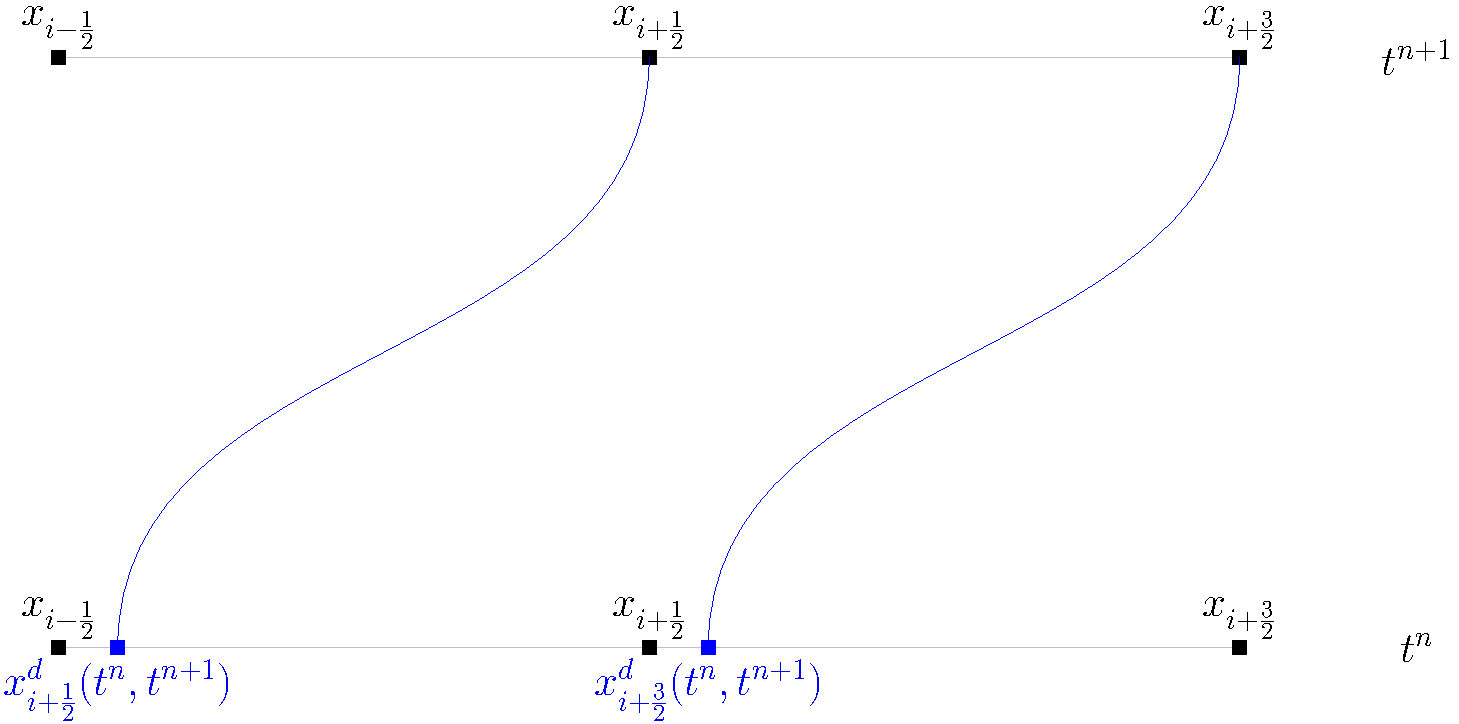
\includegraphics[width=1\linewidth]{1d_grid_departure}
	\caption{Illustration of the departure point of the cell edges from time $t^{n+1}$ to $t^n$.\label{chp-adv1d-sec1-grid1d-dep}}
\end{figure}
Integrating Equation $\eqref{chp-sec-flux:analysis-eq3}$ over the interval
$[t,s]$, we get:
\begin{equation}
	\label{chp-sec-flux:analysis-eq4}
	x^d_{i+\frac{1}{2}} (t,s) = x_{i+\frac{1}{2}} - \int_{t}^{s}u(x^d_{i+\frac{1}{2}}(\theta,s),\theta)  \,d\theta.
\end{equation}
In the following Proposition, we show how the time-averaged flux is 
related to a spatial integral over a interval depending on departure points.
\begin{prop}
	\label{chp-adv1d-sec-flux:prop1}
	Assume the framework of Problem \ref{chp-adv1d-sec2-prob2}.
	If $q$ and $u$ are $\mathcal{C}^1$ functions, then:
	\begin{align}
		\label{chp-adv1d-sec-flux:approx1}
		\int_{t^n}^{t^{n+1}} (uq)(x_{i+\frac{1}{2}},s) \,ds = 
		\int^{x_{i+\frac{1}{2}}}_{x^d_{i+\frac{1}{2}}(t^n,t^{n+1})} q(x,t^n)\,dx.
	\end{align}
\end{prop}
\begin{proof}
Using the Leibniz rule for integration (Theorem \ref{anexo-numint-lr} with 
$f(s,\theta) = u\big(x^d_{i+\frac{1}{2}}(\theta,s),\theta\big)$),
in Equation \eqref{chp-sec-flux:analysis-eq4}, it follows that:
	\begin{align}
		\begin{split}
			\label{dxds}
			{\partial_s x_{i+\frac{1}{2}}^d} (t,s) &= - \bigg({u}(x_{i+\frac{1}{2}},s) + 
			\int_{t}^{s} {\partial_s}{{u}}\big( x_{i+\frac{1}{2}}^d(\theta,s),\theta\big) \,d\theta \bigg)\\
			&=- {u}(x_{i+\frac{1}{2}},s) -
			\int_{t}^{s} {\partial_x}{{u}}\big( x_{i+\frac{1}{2}}^d(\theta, s),\theta\big) 
			{\partial_s  x_{i+\frac{1}{2}}^d}(\theta, s)\,d\theta.
		\end{split}
	\end{align}
	Taking the derivative with respect to $t$ of Equation \eqref{dxds}, we have:
	\begin{equation}
			\label{dxds_2}
			{\partial_t }{\partial_s  x_{i+\frac{1}{2}}^d}
			(t,s) = {\partial_x}{{u}}\big(x_{i+\frac{1}{2}}^d(t, s), t\big) 
			{\partial _s} x_{i+\frac{1}{2}}^d (t, s).
	\end{equation}
	Using standard ODE's techniques, 
	we get that $ x_{i+\frac{1}{2}}^d$ that solves Equations \eqref{dxds} and \eqref{dxds_2}
	is given by:
	\begin{equation}
			\label{xs_int}
			{\partial_s  x_{i+\frac{1}{2}}^d}(t,s) = -
			\exp{\bigg(\int_{t}^{s} {\partial_x}{{u}}\big( x_{i+\frac{1}{2}}^d(\theta,s),\theta\big)  \,d\theta \bigg)}
			{u}(x_{i+\frac{1}{2}},s).
	\end{equation}
	Computing $q$ on the trajectory given by $x_{i+\frac{1}{2}}^d(t,s)$ and taking
	its time derivative, we obtain:
	\begin{align}
		\label{dqdt}
		\begin{split}
			\frac{d}{dt}q\big( x_{i+\frac{1}{2}}^d(t,s),t\big) &= 
			{\partial_t}q\big( x_{i+\frac{1}{2}}^d(t,s),t\big)+
			({u}{\partial_x } 
			q)\big(x_{i+\frac{1}{2}}^d(t,s),t\big) \\
			&= -{\partial_x}{{u}}\big( x_{i+\frac{1}{2}}^d(t,s),t\big) q \big(x_{i+\frac{1}{2}}^d(t,s),t\big),
		\end{split}
	\end{align}
	where we used that $q$ satisfies the linear advection equation on its differential \eqref{chp-adv1d-sec-adv-eq1} form
   and that $x_{i+\frac{1}{2}}^d(t,s)$ solves Equation \eqref{chp-sec-flux:analysis-eq3}.
	Using again standard ODE techniques, we get that $q$ that solves Equation \eqref{dqdt}
	is given by:
	\begin{equation}
			\label{q_int}
			 q\big( x_{i+\frac{1}{2}}^d(t,s),t\big) = 
			\exp{\bigg(-\int_{t}^{s} {\partial_x}{{u}}\big( x_{i+\frac{1}{2}}^d(\theta,s),\theta\big)  \,d\theta \bigg)}
			 q(x_{i+\frac{1}{2}},s).
	\end{equation}
	Notice that if ${u}$ does not depend on $x$, then $q$ is constant along the trajectory $ x_{i+\frac{1}{2}}^d(t,s)$.
	
	Let us consider the mapping $s\in[t^n,t^{n+1}] \to  x_{i+\frac{1}{2}}^d(t^n,s)$. 
	Integrating $q$ over all departure points at time $t^n$ from $x_{i+\frac{1}{2}}$ at time $s$, we have
	\begin{equation}
		\label{depint_1}
		\int^{ x_{i+\frac{1}{2}}^d(t^n,t^{n+1})}_{ x_{i+\frac{1}{2}}^d(t^n,t^{n}) = x_{i+\frac{1}{2}}}   
		q(x,t^n)\,dx 
		= \int_{t^n}^{t^{n+1}}  q\big( x_{i+\frac{1}{2}}^d(t^n,s),t^n\big){\partial_s}{ x_{i+\frac{1}{2}}^d} (t^n,s)\,ds,
	\end{equation}
	where we are just using the variable change integration formula.
	Then, it follows from Equations  \eqref{xs_int}
	and \eqref{q_int} with $t=t^n$ that:
	\begin{equation}
		\label{depint_2}
			\int^{ x_{i+\frac{1}{2}}^d(t^n,t^{n+1})}_{x_{i+\frac{1}{2}}} q(x,t^n)\,dx 
			= -\int_{t^n}^{t^{n+1}} ({u} q)(x_{i+\frac{1}{2}},s) \,ds, 
	\end{equation}
	which is the desired formula.
\end{proof}
With the aid of Proposition \ref{chp-adv1d-sec-flux:prop1}, we can rewrite Problem \ref{chp-adv1d-sec2-prob2}
in terms of the departure point, avoiding the need for knowledge about $q$ over the
entire interval $[t^n, t^{n+1}]$. This is described in Problem \ref{chp-adv1d-sec2-prob3}:
\begin{prob}
    \label{chp-adv1d-sec2-prob3}
	\textcolor{black}{Assume the framework of Problem \ref{chp-adv1d-sec2-prob2}.
    It follows from Proposition \ref{chp-adv1d-sec-flux:prop1} that}:
\begin{equation}
	\label{1d-fvslexact-scheme}
	\begin{split}
{Q}_i(t^{n+1}) =  {Q}_i(t^{n}) -
\lambda
\bigg( \frac{1}{\Delta t}\int_{x_{i+\frac{1}{2}}^d(t^n,t^{n+1})}^{x_{i+\frac{1}{2}}}{q}(x, t^n) \,dx-
\frac{1}{\Delta t} \int_{x_{i-\frac{1}{2}}^d(t^n,t^{n+1})}^{x_{i-\frac{1}{2}}}{q}(x, t^n) \,dx \bigg),\\
\quad \forall i = 1, \ldots, N,
\quad \forall n = 0, \ldots, N_T-1,
	\end{split}
\end{equation}
	where ${Q}_i(t) = \frac{1}{\Delta x}
	\int_{x_{i-\frac{1}{2}}}^{x_{i+\frac{1}{2}}} {q}(x,t) \,dx$.
	Our problem now consists of finding the values ${Q}_i(t^{n})$, 
	$\forall i = 1, \ldots, N$, $\forall n = 0, \ldots, N_T-1$,
	given the initial values ${Q}_i(0)$, $\forall i = 1, \ldots N$.
	In other words, we would like to find the average values of ${q}$
	in each control volume $X_i$ at the considered time instants.
\end{prob}
At each time step $t^n$, we compute the values of ${Q}_i(t^{n+1})$ based on ${Q}_i(t^{n})$ and the integrals 
of $q(x, t^n)$ over specific intervals. These intervals are defined by the departure points 
$x_{i+\frac{1}{2}}^d(t^n,t^{n+1})$ and $x_{i-\frac{1}{2}}^d(t^n,t^{n+1})$.
To perform the computations, we need to determine the departure points from the edges of all control volumes
and calculate the required integrals. This idea serves as the motivation for defining finite-volume 
Semi-Lagrangian schemes. These schemes involve estimating the departure points and reconstructing the 
function $q$ at time $t^n$ using its average values $Q_i(t^n)$, which enables us to compute the necessary integrals.

\section{The finite-volume Semi-Lagrangian approach}
\label{chp-adv1d-sec2-fvsl}
Finally, we define the 1D FV-SL scheme problem as follows in Problem \ref{chp-adv1d-sec2-prob3}.
\begin{prob}[1D FV-SL scheme]
	\label{chp-adv1d-sec2-prob4}
	Assume the framework defined in Problem \ref{chp-adv1d-sec2-prob3}.
	The finite-volume Semi-Lagrangian approach of Problem \ref{chp-adv1d-sec2-prob3}
	consists of finding a scheme of the form:
	\begin{equation}
		\label{1d-fv-scheme}
		{Q}_{i}^{n+1} = {Q}_{i}^{n} -
		\lambda({F}_{i+\frac{1}{2}}^{n} - {F}_{i-\frac{1}{2}}^{n}),
		\quad \forall i = 1, \ldots, N,
		\quad \forall n = 0, \ldots, N_T-1,
	\end{equation}
	where ${Q}^{n} \in \mathbb{P}^{N}_{\nu}$ is intended to be an approximation
	of ${Q}(t^{n})\in \mathbb{P}^{N}_{\nu}$ in some sense. We define
	${Q}_{i}^{0} = {Q}_i(0)$ or ${Q}_{i}^{0} = {q}^{0}_{i}$.
	The terms ${F}_{i\pm\frac{1}{2}}^{n}$ are known as numerical flux and are given by
	\begin{equation}
		{F}_{i\pm\frac{1}{2}}^{n} =
		\frac{1}{\Delta t}
		\int_{\tilde{x}_{i\pm\frac{1}{2}}^n}^{x_{i\pm\frac{1}{2}}}\tilde{q}(x; Q^n) \,dx,
	\end{equation}
	where ${\tilde{x}_{i\pm\frac{1}{2}}}^n$ is an estimate of the departure point $x_{i-\frac{1}{2}}^d(t^n,t^{n+1})$,
	and $\tilde{q}$ is a reconstruction function for $q$ built with the values $Q^n$.
	Thus, ${F}_{i\pm\frac{1}{2}}^{n}$ approximates
	$\frac{1}{\Delta t} \int_{x_{i\pm\frac{1}{2}}^d(t^n,t^{n+1})}^{x_{i\pm \frac{1}{2}}}{q}(x, t^n) \,dx$.
\end{prob}
For a 1D FV-SL the discrete total mass at the time-step $n$ is given by
\begin{equation}
	\label{1d-fv-mass}
	M^n =  \Delta x \sum_{i=1}^N Q_i^n.
\end{equation}
Therefore, the discrete total mass is constant for a 1D-FV scheme,
which follows from a straightforward computation:
\begin{align*}
	M^{n+1} =  \Delta x \sum_{i=1}^N Q_i^{n+1}
					= M^{n} - \Delta t  \sum_{i=1}^N (F^n_{i+\frac{1}{2}}- F^n_{i-\frac{1}{2}})
					= M^{n} - \Delta t (F^n_{N+\frac{1}{2}}- F^n_{\frac{1}{2}})
					= M^{n},
\end{align*}
where we are using that $F^n_{N+\frac{1}{2}} = F^n_{\frac{1}{2}}$, since we are assuming periodic boundary
conditions.

We would like to highlight an important relationship between the average values of $q$ and
its values at the cell centroids. In Problem \ref{chp-adv1d-sec2-prob4}, we mentioned that 
the IC can be represented as $q_i^0$ instead of $Q_i(0)$.
Moreover, when analyzing the convergence of a FV-SL scheme, it is useful
to compare $Q_i^n$ with $q_i^n$ since computing $Q_i(t^n)$ requires evaluating an analytical
integral, which can be challenging in certain cases. In Proposition \ref{prop-bound-centroid},
we provide a simple proof that $q_i^n$ approximates $Q_i(t^n)$ with second-order error
when $q$ is twice continuously differentiable.
\begin{prop}
	\label{prop-bound-centroid}
	If $q \in \mathcal{C}^2_P(\Omega)$, then $Q_i(t^n)-q_i^n = C_1 \Delta x^2$, where 
	$C_1 = \frac{1}{24}\frac{\partial^2 q}{\partial x^2} (\eta, t^n)$,  $\eta \in X_i$.
\end{prop}
\begin{proof}
	Just apply Theorem \ref{prop-bound-midpoint1d} for the function $q(x,t^n)$.	
\end{proof}
Hence, 1D FV-SL schemes may be conceptualized as schemes that update the centroid values.
The Problem of the convergence of 1D FV-SL schemes is addressed in Section \ref{convergence-1dfvsl}.
Now we are going to address the problem of the departure point estimation and the reconstruction problem.

\section{Departure point computation}
\label{chp-adv1d-sec-dp}
Before presenting estimates for the departure point,
let us recall the definition of the CFL number.
\begin{definition}
	\label{chp-adv1d-sec-flux:cfl}
	For Problem \ref{chp-adv1d-sec2-prob4}, the CFL number at an edge $x_{i+\frac{1}{2}}$ and at a time level $t^n$ is defined by
	\begin{equation}
		c^n_{i+\frac{1}{2}} = \frac{\Delta t}{\Delta x}u^n_{i+\frac{1}{2}}.
	\end{equation}
\end{definition}
The CFL number is the maximum of the values $c^n_{i+\frac{1}{2}}$.
The CFL number at edges and at time levels $n+\frac{1}{2}$ is defined in the same manner.
The problem of estimating the departure point is very common in Semi-Lagrangian schemes, which are 
quite popular in atmospheric modeling. For a review of departure point calculation methods, we refer
to \citet[Chapter 3]{tumolo:2011} and the references therein. There are different approaches to compute
the departure point, such as integrating the ODE from Equation \eqref{chp-adv1d-sec-flux:prop1} using different
time integrators \citep{durran:2011} backward in time. The Runge-Kutta methods are a possible choice to 
compute the departure point (\textit{cf. e.g.} \citet{guo:2014}, \citet{lu:2022}). 

Equation \eqref{chp-sec-flux:analysis-eq4} enables us to compute or estimate the departure point.
For instance, if $u$ is constant, the departure point at time $t^n$ for the point $x_{i+\frac{1}{2}}$ at time $t^{n+1}$ is given by:
\begin{equation}
	\label{chp-sec-dp-eq1}
   x_{i+\frac{1}{2}}^d(t^n,t^{n+1}) = x_{i+\frac{1}{2}} - u\Delta t.
\end{equation}
In general, the estimated departure point, denoted by $\tilde{x}_{i+\frac{1}{2}}^n$, takes the form:
\begin{equation}
	\label{chp-sec-dp-eq2}
	\tilde{x}_{i+\frac{1}{2}}^n = x_{i+\frac{1}{2}} - \tilde{u}^{n}_{i+\frac{1}{2}}\Delta t,
\end{equation}
where $\tilde{u}^{n}_{i+\frac{1}{2}}$ represents the time-averaged wind and approximates:
\begin{equation}
	\label{chp-sec-dp-eq3}
	\frac{1}{\Delta t}\int_{t^n}^{t^{n+1}}u( x_{i+\frac{1}{2}}^d(\theta,t^{n+1}),\theta) \,d\theta.
\end{equation}
The departure point $\tilde{x}_{i+\frac{1}{2}}^n$ is said to be $p$-order accurate if:
\begin{equation}
	\label{chp-sec-dp-eq4}
	x_{i+\frac{1}{2}}^d(t^n,t^{n+1}) - \tilde{x}_{i+\frac{1}{2}}^n = \mathcal{O}(\Delta t^p).
\end{equation}

\subsection{DP1 scheme}
\label{chp-adv1d-sec-DP1}
One possible way of estimating the time-averaged wind is by using:
\begin{equation}
	\label{chp-sec-dp-eq5}
	\tilde{u}^n_{i+\frac{1}{2}} = u^{n+\frac{1}{2}}_{i+\frac{1}{2}},
\end{equation}
as in FV3 papers \citep{lin:1996,putman:2007}. 
In this case, the time-averaged CFL is given by:
\begin{equation}
	\label{chp-sec-dp-eq5b}
	\tilde{c}^n_{i+\frac{1}{2}} = c^{n+\frac{1}{2}}_{i+\frac{1}{2}}.
\end{equation}
For simplicity, in this Chapter, we shall assume that the wind is known for all time instants needed.
This scheme will be referred to as \textbf{DP1}.
In FV3, the wind is at time level $n+\frac{1}{2}$ is obtained by solving the horizontal dynamics on a C-grid as an intermediate step \citep{lin:1997,lin:2004}.
Our objective now is to determine the value of $p$ in Equation \eqref{chp-sec-dp-eq4}
in the following proposition. It is useful to introduce the concept of a material derivative beforehand:
\begin{equation*}
	\frac{Dh}{Dt} = \frac{\partial h}{\partial t} + u\frac{\partial h}{\partial x},
\end{equation*}
where $h$ is a function belonging to $\mathcal{C}^1$.
\begin{prop}
	\label{chp-sec-flux:dp_euler}
	If $u\in \mathcal{C}^1$ and the time-averaged wind is computed using Equation \eqref{chp-sec-dp-eq5}, then the departure point from Equation \eqref{chp-sec-dp-eq2} satisfies:
	\begin{equation}
         x_{i+\frac{1}{2}}^d(t^n,t^{n+1}) - \tilde{x}_{i+\frac{1}{2}}^n = \mathcal{O}(\Delta t^2).
	\end{equation}
\end{prop}
\begin{proof}
	Using the midpoint rule (Theorem \ref{prop-bound-midpoint1d}) for the function 
   $f(t) = u\big(x_{i+\frac{1}{2}}^d(t,t^{n+1}),t\big)$ in Equation \eqref{chp-sec-flux:analysis-eq4}, we obtain:
	\begin{equation}
		\label{chp-sec-flux:departurepoint4}
	   x_{i+\frac{1}{2}}^d(t^n,t^{n+1}) = x_{i+\frac{1}{2}} 
      - u\big(x_{i+\frac{1}{2}}^d (t^{n+\frac{1}{2}},t^{n+1}),t^{n+\frac{1}{2}}\big)\Delta t 
      - \frac{1}{24}\frac{D^2u}{Dt^2}\big(x_{i+\frac{1}{2}}^d(\theta_1,t^{n+1}),\theta_1\big)\Delta t^2,
	\end{equation}
	for $\theta_1 \in [t^n, t^{n+1}]$.
   Now observe that, from the intermediate value theorem for integrals and Equation \eqref{chp-sec-flux:analysis-eq4}, we have
\begin{equation*}
x_{i+\frac{1}{2}}^d(t^{n+\frac{1}{2}},t^{n+1})  =
x_{i+\frac{1}{2}} - \frac{\Delta t}{2}u\big(x_{i+\frac{1}{2}}^d(\theta_2,t^{n+1}), \theta_2 \big)
\end{equation*}
	for $\theta_2 \in [t^{n+\frac{1}{2}}, t^{n+1}]$.
   Combining this with a Taylor's expansion of $u\big(x_{i+\frac{1}{2}}^d(t,t^{n+1}),t^{n+\frac{1}{2}}\big)$ for $t = t^{n+\frac{1}{2}}$, we have:
	\begin{equation}
		\label{chp-sec-flux:departurepoint5}
		u\big(x_{i+\frac{1}{2}}^d(t^{n+\frac{1}{2}},t^{n+1}),t^{n+\frac{1}{2}}\big) = u^{n+\frac{1}{2}}_{i+\frac{1}{2}} - 
        \bigg(u\frac{\partial u}{\partial x}\bigg)\big(x_{i+\frac{1}{2}}(\theta_3,t^{n+1}),t^{n+\frac{1}{2}})\big)
        u\big(x_{i+\frac{1}{2}}^d(\theta_2,t^{n+1}), \theta_2 \big)\frac{\Delta t^2}{2},
	\end{equation}
	for $\theta_3 \in [t^n, t^{n+1}]$.
	Substituting Equation \eqref{chp-sec-flux:departurepoint5} into Equation \eqref{chp-sec-flux:departurepoint4}, we obtain the desired estimate.
\end{proof}

\subsection{DP2 scheme}
\label{chp-adv1d-sec-DP2}
In this work, we shall
consider a second-order Runge-Kutta method to compute the departure point, which we express in terms of
$\tilde{u}^n_{i+\frac{1}{2}}$ using the following equations \citep{durran:2010}:
\begin{align}
	\label{chp-sec-flux:dp_DP2}
	\tilde{x}_{i+\frac{1}{2}}^{n+\frac{1}{2}} &= x_{i+\frac{1}{2}} - u_{i+\frac{1}{2}}^n
	 \frac{\Delta t}{2} = x_{i+\frac{1}{2}} - c_{i+\frac{1}{2}}^n \frac{\Delta x}{2}, \nonumber \\
	\tilde{u}^n_{i+\frac{1}{2}} &= u\bigg(\tilde{x}^{n+\frac{1}{2}}_{i+\frac{1}{2}}, t^n + \frac{\Delta t}{2}\bigg).
\end{align}
Notice that this scheme requires values of $u$ at points that are not grid points,
both in space and time. We overcome this using linear interpolation in space:
\begin{equation}
	\tilde{u}^n_{i+\frac{1}{2}} =
	\begin{cases}
		\big(1-\alpha_{i+\frac{1}{2}}^n \big)u^{n+\frac{1}{2}}_{i+\frac{1}{2}-k} +
        \alpha_{i+\frac{1}{2}}^n u^{n+\frac{1}{2}}_{i-\frac{1}{2}-k} & \text{if } {u}^n_{i+\frac{1}{2}}\geq 0,\\
		-\alpha_{i+\frac{1}{2}}^n u^{n+\frac{1}{2}}_{i+\frac{3}{2}-k} + \big(1+\alpha_{i+\frac{1}{2}}^n\big)
        u^{n+\frac{1}{2}}_{i+\frac{1}{2}-k} & \text{if } {u}^n_{i+\frac{1}{2}} < 0,\
	\end{cases}
\end{equation}
where $\frac{c_{i+\frac{1}{2}}^n}{2} = \alpha_{i+\frac{1}{2}}^n + k$, 
$k=\lfloor \frac{c_{i+\frac{1}{2}}^n}{2} \rfloor$, $\alpha_{i+\frac{1}{2}}^n \in [0,1[$, and $\lfloor \cdot \rfloor$ is
the floor function. This scheme leads to a third-order error in the departure point estimate (\textit{cf.} \textit{e.g.} 
\citet[Section 7.1.2]{durran:2010}). This scheme shall be referred to as \textbf{DP2}.
As we mention in scheme DP1, we use the exact values of the wind needed at the time step $n+\frac{1}{2}$ and cell edge indexes $i+\frac{1}{2}$.
Notice that for this scheme, we need ghost values for the velocity, depending on how large the CFL number is.
In particular, if the CFL number is less than 2, then $k=0$ and we need the ghost values $u_{-1+\frac{1}{2}}^n$ and $u_{N+\frac{3}{2}}^n$.
In this case, it useful to work with the time-averaged CFL number:
\begin{equation}
	\label{cfl-dp2}
	\tilde{c}^n_{i+\frac{1}{2}} =
	\begin{cases}
		\bigg(1-\frac{c_{i+\frac{1}{2}}^n}{2} \bigg)c^{n+\frac{1}{2}}_{i+\frac{1}{2}} +
     \frac{c_{i+\frac{1}{2}}^n}{2} c^{n+\frac{1}{2}}_{i-\frac{1}{2}} & \text{if } {c}^n_{i+\frac{1}{2}}\geq 0,\\
		\frac{c_{i+\frac{1}{2}}^n}{2} c^{n+\frac{1}{2}}_{i+\frac{3}{2}} + \bigg(1-\frac{c_{i+\frac{1}{2}}^n}{2}\bigg)
        c^{n+\frac{1}{2}}_{i+\frac{1}{2}} & \text{if } {c}^n_{i+\frac{1}{2}} < 0.\
	\end{cases}
\end{equation}

\section{Reconstruction: the Piecewise-Parabolic Method}
\label{chp-adv1d-sec-recon}
In this Section, we will review the Piecewise-Parabolic Method (PPM).
The analysis of its accuracy will be presented in Section \ref{chp-adv1d-sec-numerical-analysis-ppm}.
PPM was originally proposed by \citet{colella:1984} for gas dynamic simulations, and its applicability
to atmospheric simulations has been demonstrated by \citet{carpenter:1990}.
This method is based on utilizing parabolas to reconstruct the function using its average values,
ensuring both mass conservation and monotonicity. PPM is an extension of the Piecewise-Linear Method
introduced by \citet{vanleer:1977}, and it is implemented in the FV3 dycore using the dimension
splitting method developed by \citet{lin:1996}.

Let's consider a function ${q}$ defined in $\Omega=[a,b]$ and a $\Delta x$-grid covering $\Omega$.
We assume that we are given the average values ${Q}_i = \frac{1}{\Delta x} \int_{x_{i-\frac{1}{2}}}^{x_{i+\frac{1}{2}}} {q}(x) \,dx$
for each control volume $X_i$, where $i = 1, \ldots, N$.
In this context, it is convenient to define the $\Delta x$-grid function $Q\in \mathbb{P}^{N}_{\nu}$ with the entries given by $Q_i$.
To facilitate the discussion, we introduce the indicator function $\chi_{i}(x)$ for each control volume $X_i$, defined as:
\begin{equation*}
	\label{chp-adv1d-sec3-1-eq1}
	\chi_{i}(x)=
	\begin{cases}
		1 & \text{if } x \in X_i,\\
		0 & \text{otherwise.}
	\end{cases}
\end{equation*}
Drawing inspiration from \citet[Chapter~1]{stoer:2002}, we consider a family of functions $\Phi(\xi;\mu)$
defined for $\xi \in [0,1]$, depending on a parameter $\mu =(\mu_0, \mu_1,\ldots, \mu_d)\in \mathbb{R}^{d+1}$.
The reconstruction problem involves finding a piecewise function:
\begin{equation}
	\label{chp-adv1d-sec3-1-eq2}
	\tilde{q}(x;Q) = \sum_{i=1}^{N} \chi_i(x) q_i(x;Q),
\end{equation}
where $q_i(x;Q) = \Phi\big(\frac{x-x_{i-\frac{1}{2}}}{\Delta x};\alpha_i\big)$ and
$\alpha_i= (\alpha_{i0},\alpha_{i1}, \ldots \alpha_{id})\in\mathbb{R}^{d+1}$. It is required that:
\begin{equation*}
	\frac{1}{\Delta x}\int_{x_{i-\frac{1}{2}}}^{x_{i+\frac{1}{2}}} \tilde{q}(x;Q) \,dx =
	\frac{1}{\Delta x}\int_{x_{i-\frac{1}{2}}}^{x_{i+\frac{1}{2}}} q_i(x;Q) \,dx =
	\int_{0}^{1} \Phi(\xi;\alpha_i) \,d\xi = {Q}_i,
\end{equation*}
which means that $q_i(x;Q)$ preserves the mass within each control volume $X_i$.

Notice that, given $q_i(x;Q) = \Phi\big(\frac{x-x_{i-\frac{1}{2}}}{\Delta x};\alpha_i\big)$, 
it is reasonable to expect that $\Phi(0;\alpha_i)$ approximates $q_i(x_{i-\frac{1}{2}})$ and
$\Phi(1;\alpha_i)$ approximates $q_i(x_{i+\frac{1}{2}})$. Additionally, if both $q$ and
$\Phi$ are sufficiently differentiable, $\Phi^{(l)}(0;\alpha_i)$ should approximate
$(\Delta x)^l q^{(l)}(x_{i-\frac{1}{2}})$ and $\Phi^{(l)}(1;\alpha_i)$ should
approximate $(\Delta x)^l q^{(l)}(x_{i+\frac{1}{2}})$, provided these derivatives exist.

One approach to estimating these values at the edges $x_{i+\frac{1}{2}}$ using the average 
values $Q$ is by employing a reconstruction method based on primitive functions \citep[Chapter~17]{leveque:2002}. 
It is worth noting that if we define:
\begin{equation}
	\label{chp-adv1d-sec-recon-ppm-eq5}
	Q(x) = \int_{a}^x q(\xi) \,d\xi,
\end{equation}
we have $Q^{(l)}(x) = q^{(l-1)}(x)$. 
Specifically, $Q^{(l)}(x_{i+\frac{1}{2}}) = q^{(l-1)}(x_{i+\frac{1}{2}})$ and 
$Q(x_{i+\frac{1}{2}}) = \Delta x\sum_{k=1}^i Q_k$, for all $i=0, \ldots, N$.
Therefore, we can employ finite-difference schemes to estimate $q^{(l-1)}(x_{i+\frac{1}{2}})$
using the $\Delta x$-grid function $Q$, given that it is assumed to be known.

Let us assume that the $l$-th derivative of $Q$ at $x_{i+\frac{1}{2}}$ is approximated using a
stencil $\mathcal{S}^{(l)}_{i+\frac{1}{2}}$ and weights $\beta^{(l)}_{k,i}$, where 
$k \in \mathcal{S}^{(l)}_{i+\frac{1}{2}}$. When $d$ is odd, we can seek a parameter
$\alpha_i \in \mathbb{R}^{d+1}$ that ensures mass conservation and approximates
$q$ and its derivatives at the edges by solving the following system:
\begin{equation}
	\label{chp-adv1d-recon-sys1}
	\begin{cases}
		\int_{0}^{1} \Phi(\xi;\alpha_i) \,d\xi &= {Q}_i,\\
		\Phi^{(l)}(0;\alpha_i) &= (\Delta x)^l \sum_{k \in 
		\mathcal{S}^{(l)}_{i-\frac{1}{2}}} \beta_{k,i}^{(l)} {Q}_k, \quad \text{for } l = 0, \ldots, d-1.
	\end{cases}
\end{equation}
If $d$ is even, similarly we look for a parameter $\alpha_i \in \mathbb{R}^{d+1}$ that solves:
\begin{equation}
	\begin{cases}
		\label{chp-adv1d-recon-sys2}
		\int_{0}^{1} \Phi(\xi;\alpha_i) \,d\xi &= {Q}_i,\\
		\Phi^{(l)}(0;\alpha_i) &= (\Delta x)^l \sum_{k \in \mathcal{S}^{(l)}_{i-\frac{1}{2}}} \beta_{k,i}^{(l)} {Q}_k, \quad \text{for } l = 0, \ldots, \frac{d}{2}-1,\\
		\Phi^{(l)}(1;\alpha_i) &= (\Delta x)^l \sum_{k \in \mathcal{S}^{(l)}_{i+\frac{1}{2}}} \beta_{k,i}^{(l)} {Q}_k, \quad \text{for } l = 0, \ldots, \frac{d}{2}-1.
	\end{cases}
\end{equation}
The reconstruction problem becomes linear when $\Phi(\xi;\mu)$ can be expressed as:
\begin{equation*}
	\Phi(\xi;\mu) = \sum_{k=0}^d \mu_k \Phi_k(\xi),
\end{equation*}
where $\Phi_k$ are functions defined on $[0,1]$. In this case, Equation 
\eqref{chp-adv1d-recon-sys1} and Equation \eqref{chp-adv1d-recon-sys2} form $(d+1)\times (d+1)$ linear systems.
It is common to assume that the $\Phi_k$'s are linearly independent.
Therefore, we have described a method that allows us to reconstruct a 
function from its average values, preserving its mass in each control volume, 
and approximating $q$ at the edges. This method works for functions $\Phi_k$
as long as they are sufficiently differentiable.
For example, choosing $d=0$ and $\Phi_0(\xi)=1$ gives us piecewise constant
functions, as used in \citet{godunov:1959}.
If we choose $d=1$, $\Phi_0(\xi)=1$, and $\Phi_1(\xi)=\xi$, we 
obtain a piecewise linear reconstruction, similar to \citet{vanleer:1977}.
For polynomial reconstruction schemes, we refer to \citet{engwirda:2016} and the references therein.


%\subsection{The Piecewise-Parabolic Method}
%\label{chp-adv1d-sec-ppm}
Hereafter, we are going the focus on the piecewise parabolic method from \citet{colella:1984} that uses $d=2$, 
$\Phi_0(\xi)=1$, $\Phi_1(\xi)=\xi$, $\Phi_1(\xi)=(1-\xi)\xi$. 
In order to follow the notation from \citet{colella:1984},
we write $\alpha_{0i} = q_{L, i}$, $\alpha_{1i} = \Delta q_i$ and $\alpha_{2i} = q_{6, i}$.
Therefore, each $q_i$ may be expressed as:
\begin{equation}
	\label{chp-adv1d-sec-recon-ppm-eq1}
	q_i(x;Q) = q_{L, i} + \Delta q_i z_i(x) + q_{6, i}z_i(x)(1-z_i(x)), 
	\quad \text{where }
	z_i(x) = \frac{x-x_{i-\frac{1}{2}}}{\Delta x},
	\quad x \in X_i,
\end{equation}
where the values $q_{L, i}$, $\Delta q_i$ and $q_{6, i}$  will be specified latter.
Note that each $z_i$ is just a normalization function that maps $X_i$ onto $[0,1]$.
It is easy to see that 
$\lim_{x \to x_{i-\frac{1}{2}}^+} {q_i(x;Q)} = q_{L, i}$.
If we define $q_{R, i} = \lim_{x \to x_{i+\frac{1}{2}}^-} {q_i(x;Q)}$,
then we have:
\begin{equation}
	\label{chp-adv1d-sec-recon-ppm-eq2}
	\Delta q_i = q_{R, i} - q_{L, i}.
\end{equation}
The average value of $q_i$ is given by:
\begin{equation}
	\label{chp-adv1d-sec-recon-ppm-eq3}
	\frac{1}{\Delta x}\int_{x_{i-\frac{1}{2}}}^{x_{i+\frac{1}{2}}} {q}_i(x;Q) \,dx
	= \frac{(q_{L,i} + q_{R,i})}{2} + \frac{q_{6,i}}{6}.
\end{equation}
Under the hypothesis of mass conservation, we have:
\begin{equation}
	\label{chp-adv1d-sec-recon-ppm-eq4}
	q_{6,i} = 6\bigg(Q_i - \frac{(q_{L,i} + q_{R,i})}{2}\bigg).
\end{equation}
Therefore, we have found the parameters $\Delta q_i$ and $q_{6, i}$ as
functions of the parameters $q_{L, i}$ and $q_{R, i}$,
such that the parabola $q_i$ from \eqref{chp-adv1d-sec3-1-eq2} 
guarantees mass conservation. To completely determine the 
parabola $q_i$, we need to set the values $q_{L, i}$ and
$q_{R, i}$, which, as we have seen, represent the limits of $q_i$ when
$x$ tends to the left and right boundaries of $X_i$, respectively.
Hence, it is natural to seek for $q_{L, i}$ as an approximation of $q(x_{i-\frac{1}{2}})$
and $q_{R, i}$ as an approximation of $q(x_{i+\frac{1}{2}})$.
As we mentioned before in after introducing Equation \eqref{chp-adv1d-sec-recon-ppm-eq5}, this is achieved
using finite-differences.

\subsection{Unlimited PPM reconstruction}
\label{chp-adv1d-sec-hord0}
This Subsection is dedicated to present the unlimited approximation of $q(x_{i-\frac{1}{2}})$ presented in \citet{colella:1984}.
An explicit expression for the approximation of $q(x_{i-\frac{1}{2}})$, denoted by $q_{i+\frac{1}{2}}$, is given by \citep{colella:1984}:
\begin{equation}
	\label{chp-adv1d-sec-recon-ppm-eq7}
	q_{i+\frac{1}{2}} = \frac{1}{2} \bigg( Q_{i+1} + Q_{i} \bigg) - \frac{1}{6} \bigg( \delta Q_{i+1} - \delta Q_{i}\bigg),
\end{equation}
where $\delta Q_{i}$ is the average slope in the $i$-th control-volume:
\begin{equation}
	\label{chp-adv1d-sec-recon-ppm-eq8}
	\delta Q_{i} = \frac{1}{2} \bigg( Q_{i+1} - Q_{i-1} \bigg).
\end{equation}
We notice that Formula \eqref{chp-adv1d-sec-recon-ppm-eq8} may be rewritten more explicitly as:
\begin{equation}
	\label{chp-adv1d-sec-recon-ppm-eq9}
	q_{i+\frac{1}{2}} = \frac{7}{12} \bigg( Q_{i+1} + Q_{i} \bigg) - \frac{1}{12} \bigg(  Q_{i+2} +Q_{i-1}\bigg).
\end{equation}
The Formula \eqref{chp-adv1d-sec-recon-ppm-eq9} is fourth-order accurate if
$q$ is at least $\mathcal{C}^4$ \citep{colella:1984}. Indeed, we
prove this later in Proposition \ref{prop:ppm-bound1}.
The expression for the values of $q_{R,i}$ and $q_{L,i}$ are given by:
\begin{align}
	\label{chp-adv1d-sec-recon-ppm-eq10}
	q_{R,i} = q_{i+\frac{1}{2}} \\
	\label{chp-adv1d-sec-recon-ppm-eq11}
	q_{L,i} = q_{i-\frac{1}{2}}.
\end{align}
During this work, we refer to this PPM scheme as \textbf{UNLIM}.
\textcolor{black}{
In FV3, the 1D advection solver input is named ``hord'' (horizontal advection method).
We note that UNLIM is not implemented in FV3, but we implemented it because, since it has no limiter, it is suitable for checking order of accuracy for the schemes investigated in this work.
For a list of reconstruction schemes available in FV3, refer to \citet{harris:2021}. One may see that the scheme hord=5 in FV3 is the closest to UNLIM, as hord=5 only applies a filter on the UNLIM flux to remove  2$\Delta x$ numerical noise}.

\subsection{Monotonic PPM reconstruction}
\label{chp-adv1d-sec-hord8}
This Subsection is dedicated to presenting a possible way of avoiding the creation of new 
extrema values in the PPM reconstruction. We are going to present an alternative scheme from \citet{lin:2004},
which was an attempt to reduce the diffusion of the original scheme \citet{colella:1984}
and is currently employed in the FV3 dynamical core \citep{harris:2021}.

Similarly to \citet{colella:1984}, \citet{lin:2004} reduces numerical oscillations
in the parabolas by defining the average slope as
\begin{equation}
	\label{chp-adv1d-sec-mono-eq4}
	\delta_m Q_{i} = 
	\max(|\delta Q_i|, 2\delta Q_{\min,i}, 2\delta Q_{\max,i}) \cdot \text{sgn}(\delta Q_i)
\end{equation}
where 
$\delta Q_i= \frac{Q_{i+1}-Q_{i-1}}{2}$,
$\delta Q_{\min,i} = Q_i - \min(Q_{i+1}, Q_i, Q_{i-1})$ 
$\delta Q_{\max,i} = \max(Q_{i+1}, Q_i, Q_{i-1}) - Q_i$.
We then initially compute an analogous version of Equation \eqref{chp-adv1d-sec-recon-ppm-eq7} as:
\begin{equation}
	q_{i+\frac{1}{2}} = 
	\frac{1}{2} \bigg( Q_{i+1} + Q_{i} \bigg) - \frac{1}{6} \bigg( \delta_m Q_{i+1} - \delta_m Q_{i}\bigg).
\end{equation}
The values $q_{R,i}$ and $q_{L,i}$ are then computed using Equations \eqref{chp-adv1d-sec-recon-ppm-eq10}
and \eqref{chp-adv1d-sec-recon-ppm-eq11}, respectively.
The monotonicity is achieved by the following scheme:
\begin{align}
	\label{chp-adv1d-sec-mono-eq5}
	q_{L,i} &\leftarrow Q_i - \max(|\delta_m Q_i|, |q_{L,i}-Q_i|) \cdot \text{sgn}(\delta_m Q_i),\\
	q_{R,i} &\leftarrow Q_i - \max(|\delta_m Q_i|, |q_{R,i}-Q_i|) \cdot \text{sgn}(\delta_m Q_i).
\end{align}
This scheme may be further improved to reduce the diffusion even more, as described by \citet{lin:2004},
but we are not going to assess this approach here.
This scheme is referred to as \textbf{MONO}.
In FV3, the paramenter ``hord'' is set equal to 8 to use this scheme.
At last, we point out again that many other PPM reconstruction schemes are available in the literature and in FV3 
\citep{harris:2021,lin:2017}, but for simplicity, we are just going to consider the schemes UNLIM and MONO.


\begin{figure}[!htb]
	\centering
	\begin{subfigure}{0.4\textwidth}
		\centering
		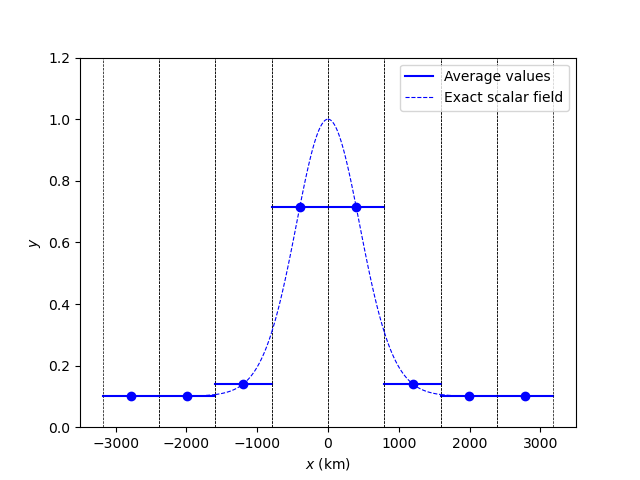
\includegraphics[width=1.12\linewidth]{ppm_recon}
		\caption{Periodic Gaussian  hill (blue dashed line) and its average values (blue horizontal lines and blue circles). \label{recon-ppm-fig-av}}
	\end{subfigure}

	\begin{subfigure}{0.4\textwidth}
		\centering
		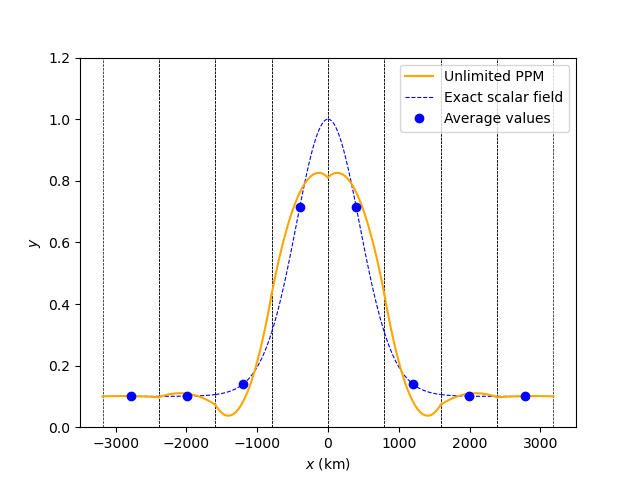
\includegraphics[width=1.12\linewidth]{ppm_recon-unlim}
		\caption{Unlimited PPM reconstruction of the periodic Gaussian  hill (yellow curve).\label{recon-ppm-fig-unlim}}
	\end{subfigure}
	\begin{subfigure}{0.4\textwidth}
		\centering
		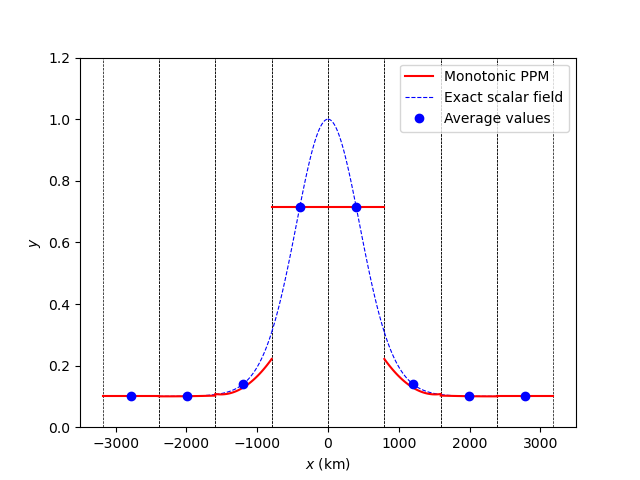
\includegraphics[width=1.12\linewidth]{ppm_recon-mono}
		\caption{Monotonic PPM reconstruction of the periodic Gaussian  hill (red curve).\label{recon-ppm-fig-mono}}
	\end{subfigure}
	\caption{
	\textcolor{red}{
    Illustration of the periodic Gaussian  hill from Equation \eqref{chp-adv1d-ic2} and its average values (a). The unlimited and monotonic PPM reconstructions are depicted in (b) and (c). We are considering $N=8$ control volumes, whose boundaries are illustrated using vertical dashed lines.\label{recon-ppm-fig}}}
\end{figure}

\textcolor{red}{
To conclude this section, we illustrate the difference between the UNLIM and MONO reconstructions using a numerical experiment. 
Following the approach in \citet{trefethen:2000}, we consider the periodic Gaussian profile defined as:
\begin{equation}
	\label{chp-adv1d-ic2}
	q(x) = 0.1 + 0.9\exp\bigg(-10\sin^2{\bigg(\frac{\pi x}{L}\bigg)}\bigg),\quad x \in \bigg[-\frac{L}{2},\frac{L}{2}\bigg],
\end{equation}
where $L = \frac{\pi}{2} R$, and $R = 6.371 \times 10^{6}$ meters is the Earth's radius.
Figure \ref{recon-ppm-fig} depicts the periodic Gaussian hill along with its average values (Figure \ref{recon-ppm-fig-av}) for $N=8$ control volumes,
with unlimited (Figure \ref{recon-ppm-fig-unlim}) and monotonic (Figure \ref{recon-ppm-fig-mono}) reconstructions. 
It is clear that the unlimited reconstruction (Figure \ref{recon-ppm-fig-unlim}) creates new extrema, which are not observed in the monotonic reconstruction (Figure \ref{recon-ppm-fig-mono}).}

\section{Flux}
\label{chp-adv1d-sec-flux}
Let us consider the framework outlined in Problem \ref{chp-adv1d-sec2-prob4}.
Assuming that $Q^{n} \in \mathbb{P}^{N}_{\nu}$ is known, our objective is to compute the values $Q^{n+1}$.
To accomplish this, we utilize a scheme similar to the one presented in Problem \ref{chp-adv1d-sec2-prob4},
taking into account the presence of a reconstruction function $\tilde{q}(x;Q^n)$ as discussed in Section
\ref{chp-adv1d-sec-recon}, and an initial departure point estimation
$\tilde{x}_{i+\frac{1}{2}}^n = {x}_{i+\frac{1}{2}} -\tilde{u}_{i+\frac{1}{2}}^n \Delta t$
for a time-averaged wind $\tilde{u}_{i+\frac{1}{2}}^n$ as explained in Section \ref{chp-adv1d-sec-dp}.
The numerical flux function ${F}^{n}_{i+\frac{1}{2}}$ is then suggested in Problem \ref{chp-adv1d-sec2-prob4}:
\begin{equation}
	\label{chp-sec-flux:numerical-flux1}
	{F}^{n}_{i+\frac{1}{2}}[Q^n,\tilde{u}^n]  = \frac{1}{\Delta t}
	\int_{x_{i+\frac{1}{2}}-\tilde{u}^n_{i+\frac{1}{2}}\Delta t}^{x_{i+\frac{1}{2}}}
	\tilde{q}(x;Q^n) \,dx.
\end{equation}
Notice that if we define the averaged CFL number,
\begin{equation*}
	\label{chp-sec-flux:cedges}
	\tilde{c}_{i+\frac{1}{2}}^n = \tilde{u}_{i+\frac{1}{2}}^n\frac{\Delta t}{\Delta x},
\end{equation*}
where $\tilde{c}_{i+\frac{1}{2}}^n = k + \alpha_{i+\frac{1}{2}}^n$, $k = \lfloor \tilde{c}_{i+\frac{1}{2}}^n \rfloor$,
$\alpha_{i+\frac{1}{2}}^n \in [0,1[$,
we can express the numerical flux as \citep{lin:1996, chen:2017}:
\begin{equation}
	\label{chp-sec-flux:numerical-flux}
	{F}_{i+\frac{1}{2}}^n[Q^n,\tilde{u}^n] =  \frac{1}{\Delta t}
	\begin{cases}
	\Delta x\sum_{l=0}^{k-1} Q_{i-l} +  
    \int_{x_{i-k+\frac{1}{2}}-{\alpha}^n_{i+\frac{1}{2}}\Delta x}^{x_{i-k+\frac{1}{2}}}
    \tilde{q}(x;Q^n) \,dx, & \text{if } \tilde{u}_{i+\frac{1}{2}}^n \geq 0,\\
	\Delta x\sum_{l=0}^{k-1} Q_{i-l} -  
    \int^{x_{i-k+\frac{1}{2}}-{\alpha}^n_{i+\frac{1}{2}}\Delta x}_{x_{i-k+\frac{1}{2}}}
    \tilde{q}(x;Q^n) \,dx, & \text{if } \tilde{u}_{i+\frac{1}{2}}^n < 0,
	\end{cases}
\end{equation}
where we used that $\tilde{q}$ preserves the local mass.

We will provide explicit expressions for the integrals in Equation \eqref{chp-sec-flux:numerical-flux} 
when using the PPM method. For each control volume edge, denoted by $i=0, \ldots, N$, and $y>0$, 
we define the following averages of the Piecewise-Parabolic approximation, as defined in
Equation \eqref{chp-adv1d-sec3-1-eq2} for $Q^{n}$ \citep{colella:1984}:
\begin{equation}
	\label{chp-sec-flux:fL_1}
	F_{L,i+\frac{1}{2}}[Q^n,y] = \frac{1}{y} \int_{x_{i+\frac{1}{2}}-y}^{x_{i+\frac{1}{2}}}
	\tilde{q}(x;Q^n)\,dx,
\end{equation}
and
\begin{equation}
	\label{chp-sec-flux:fR_1}
	F_{R,i+\frac{1}{2}}[Q^n,y] = \frac{1}{y} \int_{x_{i+\frac{1}{2}}}^{x_{i+\frac{1}{2}+y}}
	\tilde{q}(x;Q^n)\,dx.
\end{equation}
If $y \leq \Delta x$, then both of the above integral domains
are constrained to a single control volume. Thus,
it follows from a straightforward computation using 
Equation \eqref{chp-adv1d-sec-recon-ppm-eq1} that:
\begin{equation}
	\label{chp-sec-flux:fL_2}
	F_{L,i+\frac{1}{2}}[Q^n,y] = \frac{1}{y} \int_{x_{i+\frac{1}{2}}-y}^{x_{i+\frac{1}{2}}}
	q_{i}(x;Q^n)\,dx = 
	q_{R,i} +\frac{(q_{6,i} - \Delta q_i)}{2\Delta x}y
	- \frac{q_{6,i}}{3\Delta x^2}y^2,
\end{equation}
and
\begin{equation}
	\label{chp-sec-flux:fR_2}
	F_{R,i+\frac{1}{2}}[Q^n,y] = \frac{1}{y} \int_{x_{i+\frac{1}{2}}}^{x_{i+\frac{1}{2}}+y}
	q_{i+1}(x;Q^n)\,dx = 
	q_{L,i+1} +\frac{(q_{6,i+1} + \Delta q_{i+1})}{2\Delta x}y
	- \frac{q_{6,i+1}}{3\Delta x^2}y^2.
\end{equation}
The numerical flux function for PPM is then defined by:
\begin{equation}
	\label{chp-sec-flux:numerical-flux2}
        \mathfrak{F}_{i+\frac{1}{2}}^{PPM}[Q^n,\tilde{u}^n] =
    	\begin{cases} F_{L,i+\frac{1}{2}}[Q^n, {\alpha}_{i+\frac{1}{2}}^n\Delta x] & \text{if } \tilde{u}_{i+\frac{1}{2}}^n \geq 0,\\
		      F_{R,i+\frac{1}{2}}[Q^n,-{\alpha}_{i+\frac{1}{2}}^n\Delta x] & \text{if } \tilde{u}_{i+\frac{1}{2}}^n<0,
    	\end{cases}
\end{equation}
and
\begin{equation}
	\label{chp-sec-flux:numerical-flux3}
         {F}_{i+\frac{1}{2}}^n[Q^n,\tilde{u}^n]  =  \frac{1}{\Delta t} \bigg(
    	\Delta x\sum_{l=0}^{k-1} Q_{i-l} +  
        \Delta x {\alpha}_{i+\frac{1}{2}}^n\mathfrak{F}_{i+\frac{1}{2}}^{PPM}[Q^n,\tilde{u}^n]\bigg).\\
\end{equation}
%where $\tilde{u}_{i+\frac{1}{2}}^n$ is the velocity used in the departure point estimation.
In particular, if the CFL number is less than one, then:
\begin{equation}
	\label{chp-sec-flux:numerical-flux4}
        \mathfrak{F}_{i+\frac{1}{2}}^{PPM}[Q^n,\tilde{c}^n]  =  
    	\begin{cases}
        q_{R,i} +
        \big(\frac{{q_{6,i} - \Delta q_i}}{2}\big){\tilde{c}_{{i+\frac{1}{2}}}^n}
	- \frac{q_{6,i}}{3}{(\tilde{c}_{{i+\frac{1}{2}}}^n})^2, 
	& \text{if } \tilde{c}_{i+\frac{1}{2}}^n \geq 0,\\
	q_{L,i+1} +
	\big(\frac{q_{6,i+1} + \Delta q_{i+1}}{2}\big){\tilde{c}_{{i+\frac{1}{2}}}^n}
	-\frac{q_{6,i+1}}{3}({\tilde{c}_{{i+\frac{1}{2}}}^n})^2,
	& \text{if } \tilde{c}_{i+\frac{1}{2}}^n<0,
    	\end{cases}
\end{equation}
and
\begin{equation}
	\label{chp-sec-flux:numerical-flux5}
         {F}_{i+\frac{1}{2}}^{n}[Q^n,\tilde{c}^n] = 
         {\tilde{u}}_{i+\frac{1}{2}}^n\mathfrak{F}_{i+\frac{1}{2}}^{PPM}[Q^n,\tilde{c}^n],\\
\end{equation}
where we are expressing the flux in terms of the time-averaged CFL number $\tilde{c}^n$.
Notice that this flux is upwind based, that is, it always computes the flux using the parabola in the upwind direction.
Finally, for both unlimited PPM and monotonic PPM schemes, $F_{i+\frac{1}{2}}^n$ uses the stencil
$\mathcal{S}_{i+\frac{1}{2}} = \{i-3,i-2,i-1,i,i+1,i+2,i+3\}$, and therefore we need $\nu=3$ layers of ghost cells.

In FV3, the 1D flux is computed based on the perturbation values \citep{harris:2021} given by:
\begin{align}
\label{chp-sec-flux:numerical-flux6}
b_{L,i} = q_{L,i} - Q_i^n, \\
\label{chp-sec-flux:numerical-flux7}
b_{R,i} = q_{R,i} - Q_i^n.
\end{align}
Then, Equation \eqref{chp-sec-flux:numerical-flux4} becomes:
\begin{equation}
	\label{chp-sec-flux:numerical-flux8}
        \mathfrak{F}_{i+\frac{1}{2}}^{PPM}[Q^n,\tilde{c}^n]  =  
    	\begin{cases}
        Q_{i}^n +
        (1-\tilde{c}_{{i+\frac{1}{2}}}^n)
        \big(b_{R,i}-\tilde{c}_{{i+\frac{1}{2}}}^n
        (b_{L,i}+b_{R,i})\big),
	& \text{if } \tilde{c}_{i+\frac{1}{2}}^n \geq 0,\\
	Q_{i+1}^n +
        (1+\tilde{c}_{{i+\frac{1}{2}}}^n)
        \big(b_{L,i+1}+\tilde{c}_{{i+\frac{1}{2}}}^n
        (b_{L,i+1}+b_{R,i+1})\big),
	& \text{if } \tilde{c}_{i+\frac{1}{2}}^n<0,
    	\end{cases}
\end{equation}
which is the formula implemented in FV3.
Finally, the average value update is implemented in FV3 as
\begin{equation}
	\label{chp-sec-flux:numerical-flux9}
	Q_i^{n+1} = Q_i^{n} - 
        \big(\tilde{c}_{i+\frac{1}{2}}^n\mathfrak{F}_{i+\frac{1}{2}}^{PPM}[Q^n,\tilde{c}^n] -
        \tilde{c}_{i-\frac{1}{2}}^n\mathfrak{F}_{i-\frac{1}{2}}^{PPM}[Q^n,\tilde{c}^n]  \big),
\end{equation}
for $i=1, \cdots, N$.
Thefore, at each time-step, we need to:
\begin{enumerate}
\item Compute $\tilde{c}_{i+\frac{1}{2}}^n$ (for $i = 0, \cdots, N$) using the schemes DP1 or DP2;
\item Compute $q_{L,i}$ and  $q_{R,i}$ (for $i = 1, \cdots, N$) using UNLIM or MONO;
\item Evalute the pertubation values (for $i = 1, \cdots, N$) using Equations
\eqref{chp-sec-flux:numerical-flux6} and \eqref{chp-sec-flux:numerical-flux7};
\item Evaluate the fluxes  $\mathfrak{F}_{i+\frac{1}{2}}^{PPM}$ (for $i = 0, \cdots, N$) using Equation \eqref{chp-sec-flux:numerical-flux8};
\item Update the average values $Q^{n+1}$ using Equation \eqref{chp-sec-flux:numerical-flux9}.
\end{enumerate}
\section{Numerical experiments}
\label{chp-adv1d-sec-numerical-exp}
This Section is dedicated to presenting the numerical results of the PPM and 
its variations discussed here. We will consider the reconstruction
schemes unlimited PPM  (Subsection \ref{chp-adv1d-sec-hord0}) and monotonic PPM
(Subsection \ref{chp-adv1d-sec-hord8}), as well as the departure point schemes
\textbf{DP1} (Subsection \ref{chp-adv1d-sec-DP1}) and \textbf{DP2} (Subsection \ref{chp-adv1d-sec-DP2}).
The code used in this Section can be found in Appendix \ref{anexo-code}.

For all the simulations presented here, we will consider the spatial domain $[-\frac{L}{2},\frac{L}{2}]$,
and the time interval $[0,T]$,  where $L = \frac{\pi}{2} R$, $R = 6.371 \times 10^{6}$ meters is the Earth's radius and
$T = 1036800$ seconds, equivalent to 12 days.
The spatial domain spans approximately $10^4$ kilometers, which corresponds to approximately the length of a cubed-sphere panel,
as shall be seen in Chapter \ref{chp-cs-grids}.
The relative change at time step $n$ in the mass is computed as:
\begin{equation*}
	\frac{|M^n-M^0|}{|M^0|},
\end{equation*}
where $M^n$ is given by Equation \eqref{1d-fv-mass}.
For all the simulations, the
mass is preserved with machine precision. Furthermore,
we compute the initial average values $Q_i(0)$ using
the initial values of $q^0_i$ at the control volume centroids for all simulations,
which is second-order accurate by Proposition \ref{prop-bound-centroid}. 
In the error calculation, only when $q_0$ is given by Equation \eqref{chp-adv1d-ic2},
we replace $Q_{i}(t^n)$ by its centroid value $q_{i}(t^n)$, which again gives
a second-order approximation by Proposition \ref{prop-bound-centroid}.

\subsection{Square wave with constant wind advection}
\label{chp-adv1d-sec-numerical-exp-1}
As a first numerical experiment, we consider
a discontinuous IC given by:
\begin{equation}
	\label{chp-adv1d-ic1}
		q_0(x) =  
  \begin{cases}
		1 & \text{if } x \in [-0.1L,0.1L],\\
		0.1 & \text{otherwise}.
  \end{cases}
\end{equation}
for the linear advection equation with constant velocity, which we adopt as $u=\frac{L}{T}$.
\begin{figure}[!htb]
	\centering
	\includegraphics[width=0.6\linewidth]{adv1d_tc1_N48_hord8_DP1_t12}
	\caption{Linear advection experiment using the IC given by Equation \eqref{chp-adv1d-ic1} (black curve) with constant velocity.
		These figures show the advected profile after 12 days (one time period).
		Reconstruction schemes employed: unlimited PPM (UNLIM - blue curve) and monotonic PPM (MONO - orange curve).\label{chp-adv1d-sec-exp-adv1}}
\end{figure}

It is easy to check that the exact solution of Problem \ref{chp-adv1d-sec2-prob1} is given
by $q_0(x-ut)$ and that the solution returns to its initial position after 12 days.
We will employ a time step of 14400 seconds and set $N=48$ (therefore $\Delta x \approx$ 208 km) resulting in a CFL number approximately equal to 0.67.
The departure schemes \textbf{DP1} and \textbf{DP2} compute the departure point exactly in this case, so we will only use the \textbf{DP1} scheme.

In Figure \ref{chp-adv1d-sec-exp-adv1}, we present the obtained results.
It is evident that the monotonic PPM exhibit a significant advantage.
This scheme effectively prevent the strong oscillations observed in the unlimited PPM scheme,
as well as the generation of new extrema, which aligns with our expectations.

\subsection{Flow deformation with divergent wind}
\label{chp-adv1d-sec-numerical-exp-2}
As a second experiment, we shall investigate the how the PPM schemes behave when the velocity
is variable.
This cases is useful to assess the departure point schemes, which shall not be exact as in the previous test.
We are going to consider the velocity
\begin{equation}
	\label{chp-adv1d-vel2}
	u(x,t) = u_0\cos{\bigg(\frac{\pi t}{T}\bigg)}\cos^2\bigg(\pi \bigg(\frac{x}{L}-\frac{t}{T}\bigg)\bigg) + u_1.
\end{equation}
We adopt the parameters $T = 12$ days and  $u_0 = u_1 = \frac{L}{T}$.
\textcolor{red}{We set the periodic Gaussian profile defined in Equation $\eqref{chp-adv1d-ic2}$ as the initial condition.}
The velocity function given by Equation \eqref{chp-adv1d-vel2} is based
on the deformational flow test case in \citet{nair:2010},
where we add a constant wind $u_1$ to prevent error cancellations.
As the velocity is variable, we utilize the departure point schemes DP1 and DP2.
In this case, the solution exhibits a period of 12 days,
meaning that the profile deforms and returns to its initial shape
and position after 12 days, allowing us to compute the error.
Indeed, in Figure \ref{chp-adv1d-sec-exp-adv2}, we show how the solution behaves
using a high-resolution ($N=768$), the MONO scheme and the DP1 departure point scheme.
\begin{figure}[!htb]
	\centering
	\begin{subfigure}{0.3\textwidth}
		\centering
		\includegraphics[width=1.12\linewidth]{adv1d_tc3_N768_hord8_DP1_t0}
		\caption{$t=0$.\label{chp-adv1d-sec-exp-adv2-a}}
	\end{subfigure}
	\begin{subfigure}{0.3\textwidth}
		\centering
		\includegraphics[width=1.12\linewidth]{adv1d_tc3_N768_hord8_DP1_t2}
		\caption{$t=2$ days.\label{chp-adv1d-sec-exp-adv2-b}}
	\end{subfigure}
	\begin{subfigure}{0.3\textwidth}
		\centering
		\includegraphics[width=1.12\linewidth]{adv1d_tc3_N768_hord8_DP1_t4}
		\caption{$t=4$ days.\label{chp-adv1d-sec-exp-adv2-c}}
	\end{subfigure}
	
	\begin{subfigure}{0.3\textwidth}
		\centering
		\includegraphics[width=1.12\linewidth]{adv1d_tc3_N768_hord8_DP1_t6}
		\caption{$t=6$ days.\label{chp-adv1d-sec-exp-adv2-d}}
	\end{subfigure}
	\begin{subfigure}{0.3\textwidth}
		\centering
		\includegraphics[width=1.12\linewidth]{adv1d_tc3_N768_hord8_DP1_t8}
		\caption{$t=8$ days.\label{chp-adv1d-sec-exp-adv2-e}}
	\end{subfigure}
	\begin{subfigure}{0.3\textwidth}
		\centering
		\includegraphics[width=1.12\linewidth]{adv1d_tc3_N768_hord8_DP1_t10}
		\caption{$t=10$ days.\label{chp-adv1d-sec-exp-adv2-f}}
	\end{subfigure}

	\begin{subfigure}{0.3\textwidth}
		\centering
		\includegraphics[width=1.12\linewidth]{adv1d_tc3_N768_hord8_DP1_t12}
		\caption{$t=12$ days.\label{chp-adv1d-sec-exp-adv2-g}}
	\end{subfigure}
	\caption{Linear advection experiment using the velocity from Equation \eqref{chp-adv1d-ic2},
		a CFL number equal to $0.67$, $N=768$ cells, and the IC is given by 
		Equation \eqref{chp-adv1d-ic2}.
		These figures show the advected profile at
		day 0  \eqref{chp-adv1d-sec-exp-adv2-a} and after
		2 \eqref{chp-adv1d-sec-exp-adv2-b}, 
		4  \eqref{chp-adv1d-sec-exp-adv2-c},
		6  \eqref{chp-adv1d-sec-exp-adv2-d},
		8  \eqref{chp-adv1d-sec-exp-adv2-e},
		10  \eqref{chp-adv1d-sec-exp-adv2-f},
		and 12  \eqref{chp-adv1d-sec-exp-adv2-g} days.
		We are using the monotonic PPM scheme with the DP1 departure point scheme. \label{chp-adv1d-sec-exp-adv2}}
\end{figure}
\begin{figure}[!htb]
	\centering
	\begin{subfigure}{0.45\textwidth}
		\centering
		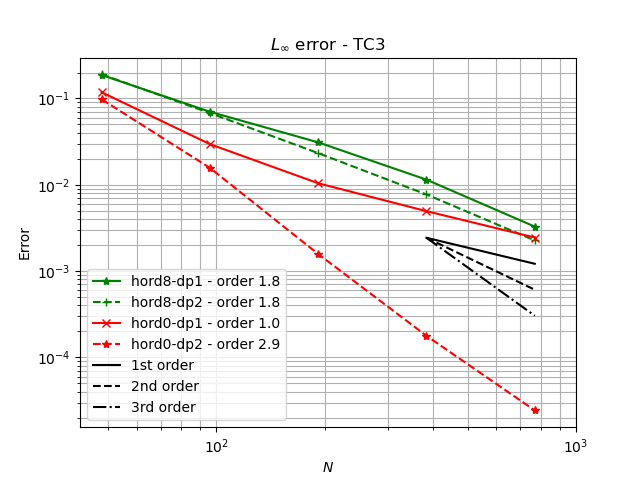
\includegraphics[width=1.12\linewidth]{adv1d_tc3_linf_error}
		\caption{$L_{\infty}$ error.\label{chp-adv1d-sec-exp-adv2-error-linf}}
	\end{subfigure}
	\begin{subfigure}{0.45\textwidth}
		\centering
		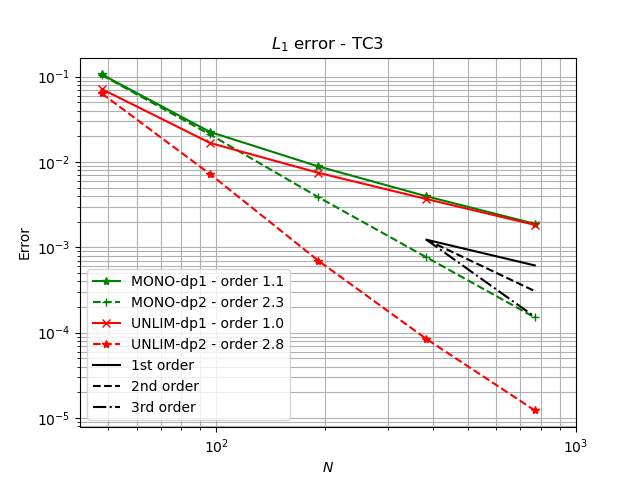
\includegraphics[width=1.12\linewidth]{adv1d_tc3_l1_error}
		\caption{$L_1$ error.\label{chp-adv1d-sec-exp-adv2-error-l1}}
	\end{subfigure}
	\caption{Relative error for the unlimited PPM (UNLIM -red lines) and monotonic PPM (MONO - green lines) schemes
	         in $L_{\infty}$
	         (Figure \ref{chp-adv1d-sec-exp-adv2-error-linf})
	         and $L_1$ norms
                 (Figure \ref{chp-adv1d-sec-exp-adv2-error-l1}).
	        Results using DP1 scheme uses solid lines and DP2 results uses dashed lines.
		The IC given by Equation
		\eqref{chp-adv1d-ic2} and the variable 
		velocity given by Equation \eqref{chp-adv1d-vel2}.\label{chp-adv1d-sec-exp-adv2-2}}
\end{figure}

To investigate the error convergence, we employ $(\Delta x^{(k)}, \Delta t^{(k)}, \lambda)$-discretizations with $\Delta x^{(k)} = \frac{L}{N^{(k)}}$,
$N^{(k)} = 48 \times 2^k$,
$\Delta t^{(k)}=\frac{7200}{{2^{k}}}$, for $k = 0, \ldots, 4$.
To measure the accuracy, we consider the relative error in the $p$-norm as follows:
\begin{equation*}
	E_k = 
	\frac{\| Q^{N_T} - Q^0 \|_{p, \Delta x}}{\|Q^0\|_{p, \Delta x}}.
\end{equation*}
We are going to consider $p=1$ and $p=\infty$.
The convergence rate is defined by
\begin{equation*}
	CR_k = \frac{\ln{\bigg(\frac{E_{k}}{E_{k-1}}}\bigg)}{\ln 2}, \quad \text{for} \quad k = 1, \ldots 4.
\end{equation*}
The difference between the DP1 and DP2 schemes becomes clear when observing the relative error in Figure \ref{chp-adv1d-sec-exp-adv2-2}.
In the $L_{\infty}$ norm (Figure \ref{chp-adv1d-sec-exp-adv2-error-linf}), 
for  the unlimited PPM, the DP1 scheme results in a first-order error in the departure point, which dominates the total error.
This observation is in agreement with the discussion in Section \ref{chp-adv1d-sec-dp}.
On the other hand, when employing the DP2 scheme, we can achieve third-order accuracy for the unlimited PPM.
For the monotonic PPM, the DP2 slightly reduces the $L_{\infty}$ error.

However, in the $L_1$ norm, as shown in Figure \ref{chp-adv1d-sec-exp-adv2-error-l1}, 
for both unlimited PPM and monotonic PPM, we observe that DP1 results in a 1st order accuracy, 
while DP2 results in schemes with an order greater than 2.
This experiment illustrates the impact of departure point calculation errors on the overall error and the benefit of using DP2.

\section{Concluding remarks}
\label{chp-adv1d-sec-conclusion}
In this Chapter, we provided a general overview of 1D FV-SL schemes for the advection equation.
We discussed the three essential tasks involved in these schemes.
The first task is the reconstruction of a function from its average values.
We employed the PPM method introduced by \citet{colella:1984}
without limiter and its monotonic variant such as the one from \citet{lin:2004}.
The second task involves computing the departure point of the control volume edges. For this purpose, 
we utilized the first-order departure point calculation  using a time-centered wind in an approach known as DP1.
Additionally, we explored a second-order approach by employing a two-stages Runge-Kutta scheme
to integrate the departure point ODE.
Lastly, the third task entails computing the flux, which involves integrating the 
reconstructed function over a domain determined by the departure point.

The difference between the departure point schemes became apparent when we performed a test 
with variable velocity. The simulation using the DP1 scheme with the unlimited PPM resulted in a final first-order 
error, despite the scheme having third-order accuracy in space. However, the DP2 scheme  with the unlimited PPM
preserved third-order accuracy despite being only second-order accurate. We expect that, in 
general, combining PPM with the DP2 scheme should result in at least second-order accuracy.
The DP2 scheme also showed to lead to a more accurate result when combined with monotonic PPM, especially in the $L_1$ norm.
Clearly, the DP2 scheme is more computationally expensive since it requires linear interpolation of the velocity field, but this additional cost is minimal.
%One possible way to reduce 
%its cost would be to use larger CFL numbers allowed by the FV-SL schemes, as discussed in 
%Section \ref{chp-adv1d-sec-flux}.
